\chapter{Implementacja} \label{chap:implementation}

\section{Opis modelu danych do reprezentacji skrzyżowań}

Drogi są reprezentowane w sposób dyskretny. Każda droga zaczyna się w pozycji 1 i rośnie wraz z jej rozmiarem. 
\newline
\newline
Samochody mogą poruszać się w następujących kierunkach:
\newline
- z północy na południe
\newline
- z południa na północ
\newline
- ze wschodu na zachód
\newline
- z zachodu na wschód
\newline
\newline
Droga jest reprezentowana poprzez następujące dane:
\newline
- unikalny numer drogi
\newline
- rozmiar drogi
\newline
- informacja o przecięciach z innymi drogami
\newline
- kierunek w którym samochód się porusza na drodze (z północy na południe, czy z południa na północ lub z zachodu na wschód czy ze wschodu na zachód)
\newline
\newline
Samochody na drogach opisują następujące dane:
\newline
- unikalny numer samochodu
\newline
- unikalny numer drogi, na której się znajduje
\newline
- numer pozycji na drodze, na której samochód się znajduje
\newline
- prędkość początkowa
\newline
- numer pozycji docelowej na drodze - punkt za ostatnim skrzyżowaniem
\newline
\newline
Samochody poruszają się po drogach w krokach czasowych. Prędkość samochodu wyrażana jest w liczbie odcinków drogi w jednym kroku czasowym.
\newline
\newline
W Systemie można wybrać maksymalne przyspieszenia ujemne oraz dodatnie samochodów z następujących możliwości \{-2, -1, 0, 1, 2\}. Oznacza to, że w następnym stanie pojazd może przyspieszyć o 1 lub 2 odcinki drogi na jeden krok czasowy. Dla wartości 0 pojazd utrzymuje swoją prędkość. Dla wartości ujemnych pojazd zwalnia o 1 lub 2 odcinki drogi na jeden kroku czasowym.
\newline
\newline
W Systemie jest także plik konfiguracyjny, który wyznacza maksymalną prędkość, oraz gdzie definiuje się wyżej opisane wartości przyspieszeń.

\section{Generyczny, wielostanowy algorytm A*}

Zaprezentowny w tej pracy zmodyfikowany algorytm A* jest algorytmem wielostanowym. Oznacza to, że wierzchołkiem w grafie jest stan wszystkich samochodów na skrzyżowaniu, a krawędzią jest przejście z jednego stanu do następnego.
\newline
\newline
Algorytm ma za zadanie doprowadzić do zadanego celu otrzymując określone dane początkowego. Stanem początkowym jest startowe rozstawienie aut na drogach.
\newline
\newline
Algorytm otrzymując dane startowe, ma osiągnąć zadany cel. Danymi startowymi jest początkowe rozstawienie samochodów na skrzyżowaniach wraz z ich początkowymi prędkościami.
\newline
\newline
Modyfikacja Algorytm A* jest generyczna. Do algorytmu przekazujemy klasę reprezentującą wierzchołek, która implementuje metodę 'neighbours', która zwraca sąsiednie wierzchołki.
\newline
\newline
Do algorytmu przekazuje się także warunki wygranej. W przypadku mojego rozwiązania wygraną jest przekroczenie przez wszystkie samochody ostatniego skrzyżowania na drogach, na których się znajdują.
\newline
\newline
Do algorytmu przekazywana jest także funkcja heurystyki, zależna od danych danego wierzchołka.

\section{Reprezentacja wierzchołka w zmodyfikowanym algorytmie A*}

Wierzchołek w modyfikacji algorytmu A* przedstawionej w tej pracy opisuje stan wszystkich samochodów na skrzyżowaniach wraz z ich prędkościami.
\newline
\newline
Zgodnie z wcześniej generycznością wierzchołek jest obiektem klasy, który implementuje metodę 'neighbours'. Metoda generuje wszystkie stany sąsiednie dla aktualnego stanu. Dla przykładu, dla ustawień przyspieszeń \{-2, -1, 0, 1, 2\}, dla każdego z aut na skrzyżowaniu generowane są stany z jego prędkością dodając wartości przyspieszeń. Pomijane są stany, w których prędkość samochodu byłaby ujemna.
\newline
\newline
W metodzie usuwane są także stany powodujące kolizje, co będzie opisane w następnym rozdziale.

\section{Unikanie kolizji}

Koniecznym elementem w planowaniu ruchu jest unikanie kolizji.
\newline
\newline
Unikanie kolizji zostało podzielone na dwa etapy
\newline
- Unikanie kolizji aut poruszających się po tym samym pasie
\newline
- Unikanie kolizji na skrzyżowaniach
\newline
\newline
Impementacja unikania kolizji pojazdów na tym samym pasie polega na policzeniu obszarów dla samochodów znajdujących się na tym samym pasie, który będą one obejmowały w jednym kroku czasowym.
\newline
\newline
Jeżeli obszary dwóch samochdów na jednym pasie pokrywają się - taki stan jest usuwany i wówczas metoda 'neighbours' nie zwróci go jako stanu sąsiedniego.
\newline
\newline
Unikanie kolizji na skrzyżowaniach polega na eliminacji stanów, w których conajmniej dwa auta przekroczyły w jednym kroku czasowym to samo skrzyżowanie. Metoda 'neighbours' także nie zwróci takich stanów.

\section{Funkcja heurystyki}

Funkcja heurystyki dla algorytmu A* jest to suma kroków czasowych, po których wszystkie auta przekroczą ostatnie skrzyżowanie - czyli osiągną cel. Funkcja liczona jest, przy założeniu, że wszystkie samochody maksymalnie przyspieszają.

\section{Reprezentacja graficzna wyników}

W celu graficznej reprezentacji wyników zaimplementowany został moduł graficzny.
\newline
\newline
Działanie modułu graficznego oparte jest na rysowaniu grafów z wykorzystaniem biblioteki Graphviz oraz jej implementacji w języku Ruby.
\newline
\newline
Skrzyżowanie jest reprezentowane za pomocą grafu. Wierzchołkami grafu są poszczególne odcinki dróg. Krawędziami grafu są połączenia pomiędzy odcinkami.
\newline
\newline
Każda droga jest oznaczona innym kolorem.
\newline
\newline
Samochody poruszające się po tej samej drodze są zaznaczone grubszym obwodem oraz mają ten sam kolor. Samochody można rozróżnić poprzez unikalny numer na nich napisany.
\newline
\newline
Kolejne kroki czasowe reprezentowane są poprzez następne grafy z kolejnymi ułożeniami samochodów.
\newline
\newline
Ostatnim elementem modułu graficznego jest stworzenie GIFa z następujących po sobie grafów.
\newline
\newline
Poniżej na rysunkach \ref{1-traffic} - \ref{12-traffic} jest przedstawione zostało rozwiązanie dla dwunastu pojazdów na skrzyżowaniu ośmiu dróg.
\newline
Jak widać na rysunku \ref{12-traffic} po dwunastym kroku czasowym wszystkie samochody opóściły skrzyżowanie.
\newpage
\begin{figure}
    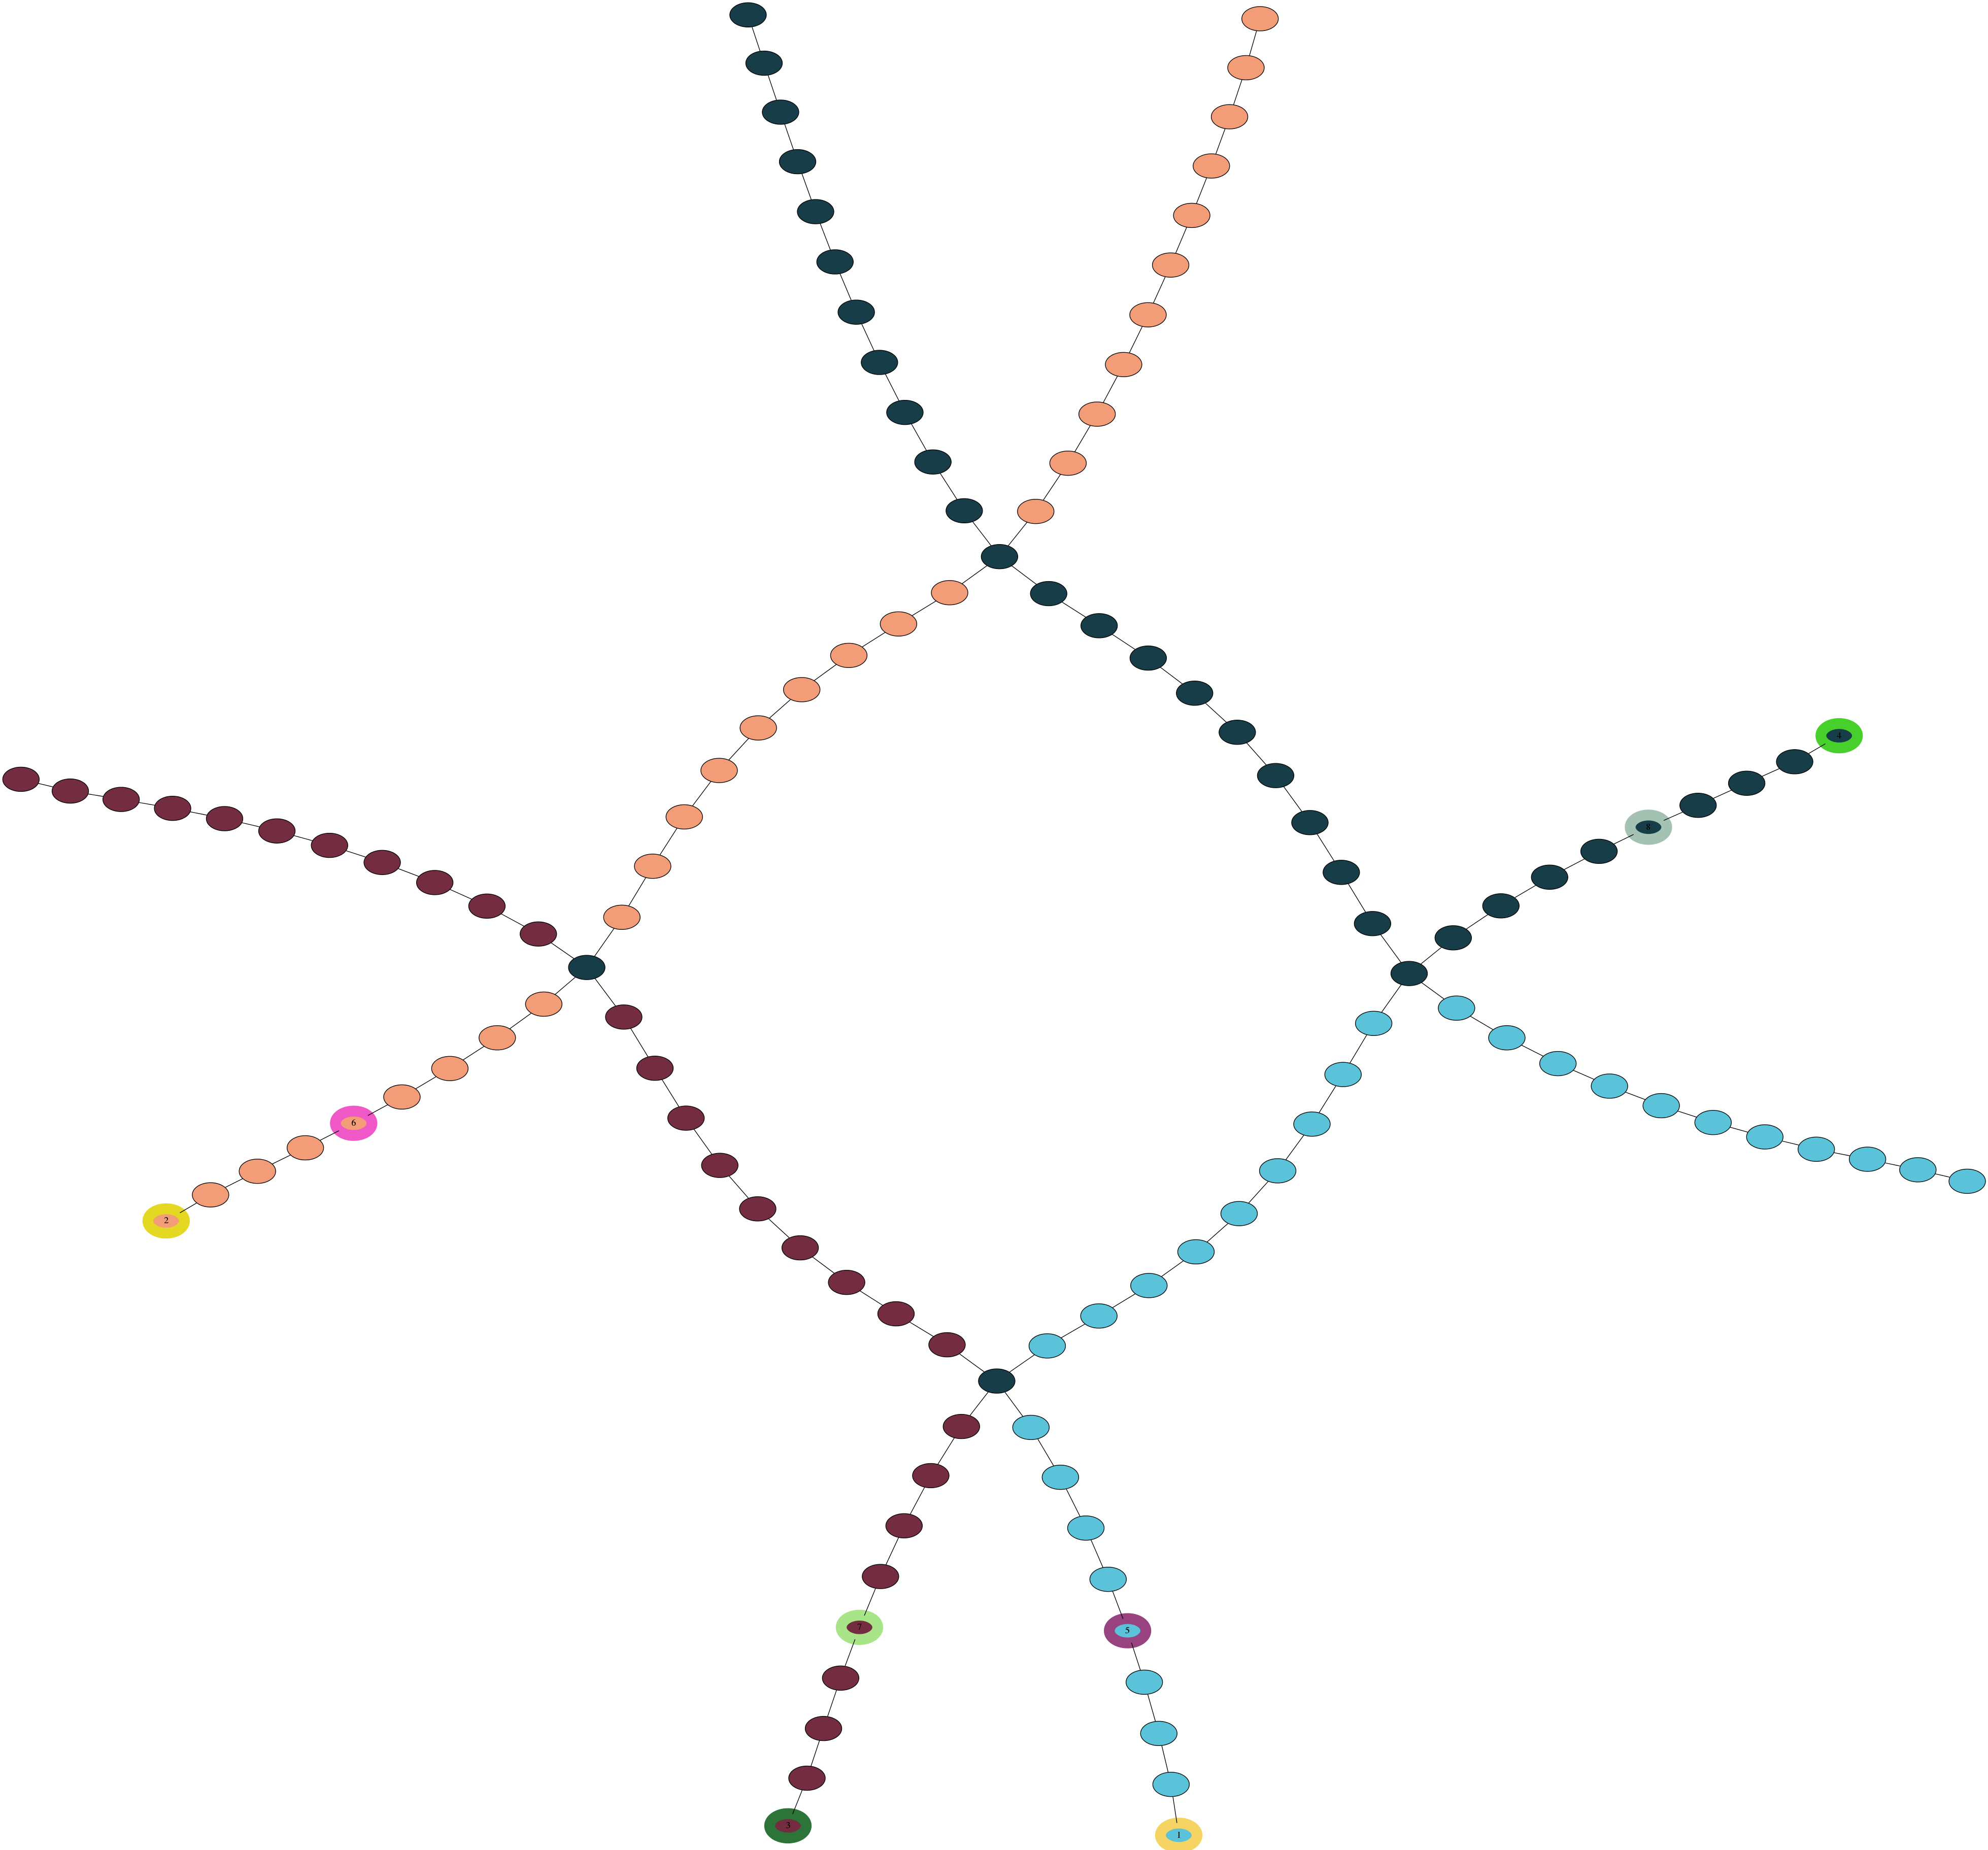
\includegraphics[width=1.0\textwidth]{1.png}
  \caption{1 krok czasowy}
  \label{1-traffic}
\end{figure}
\newpage
\begin{figure}
    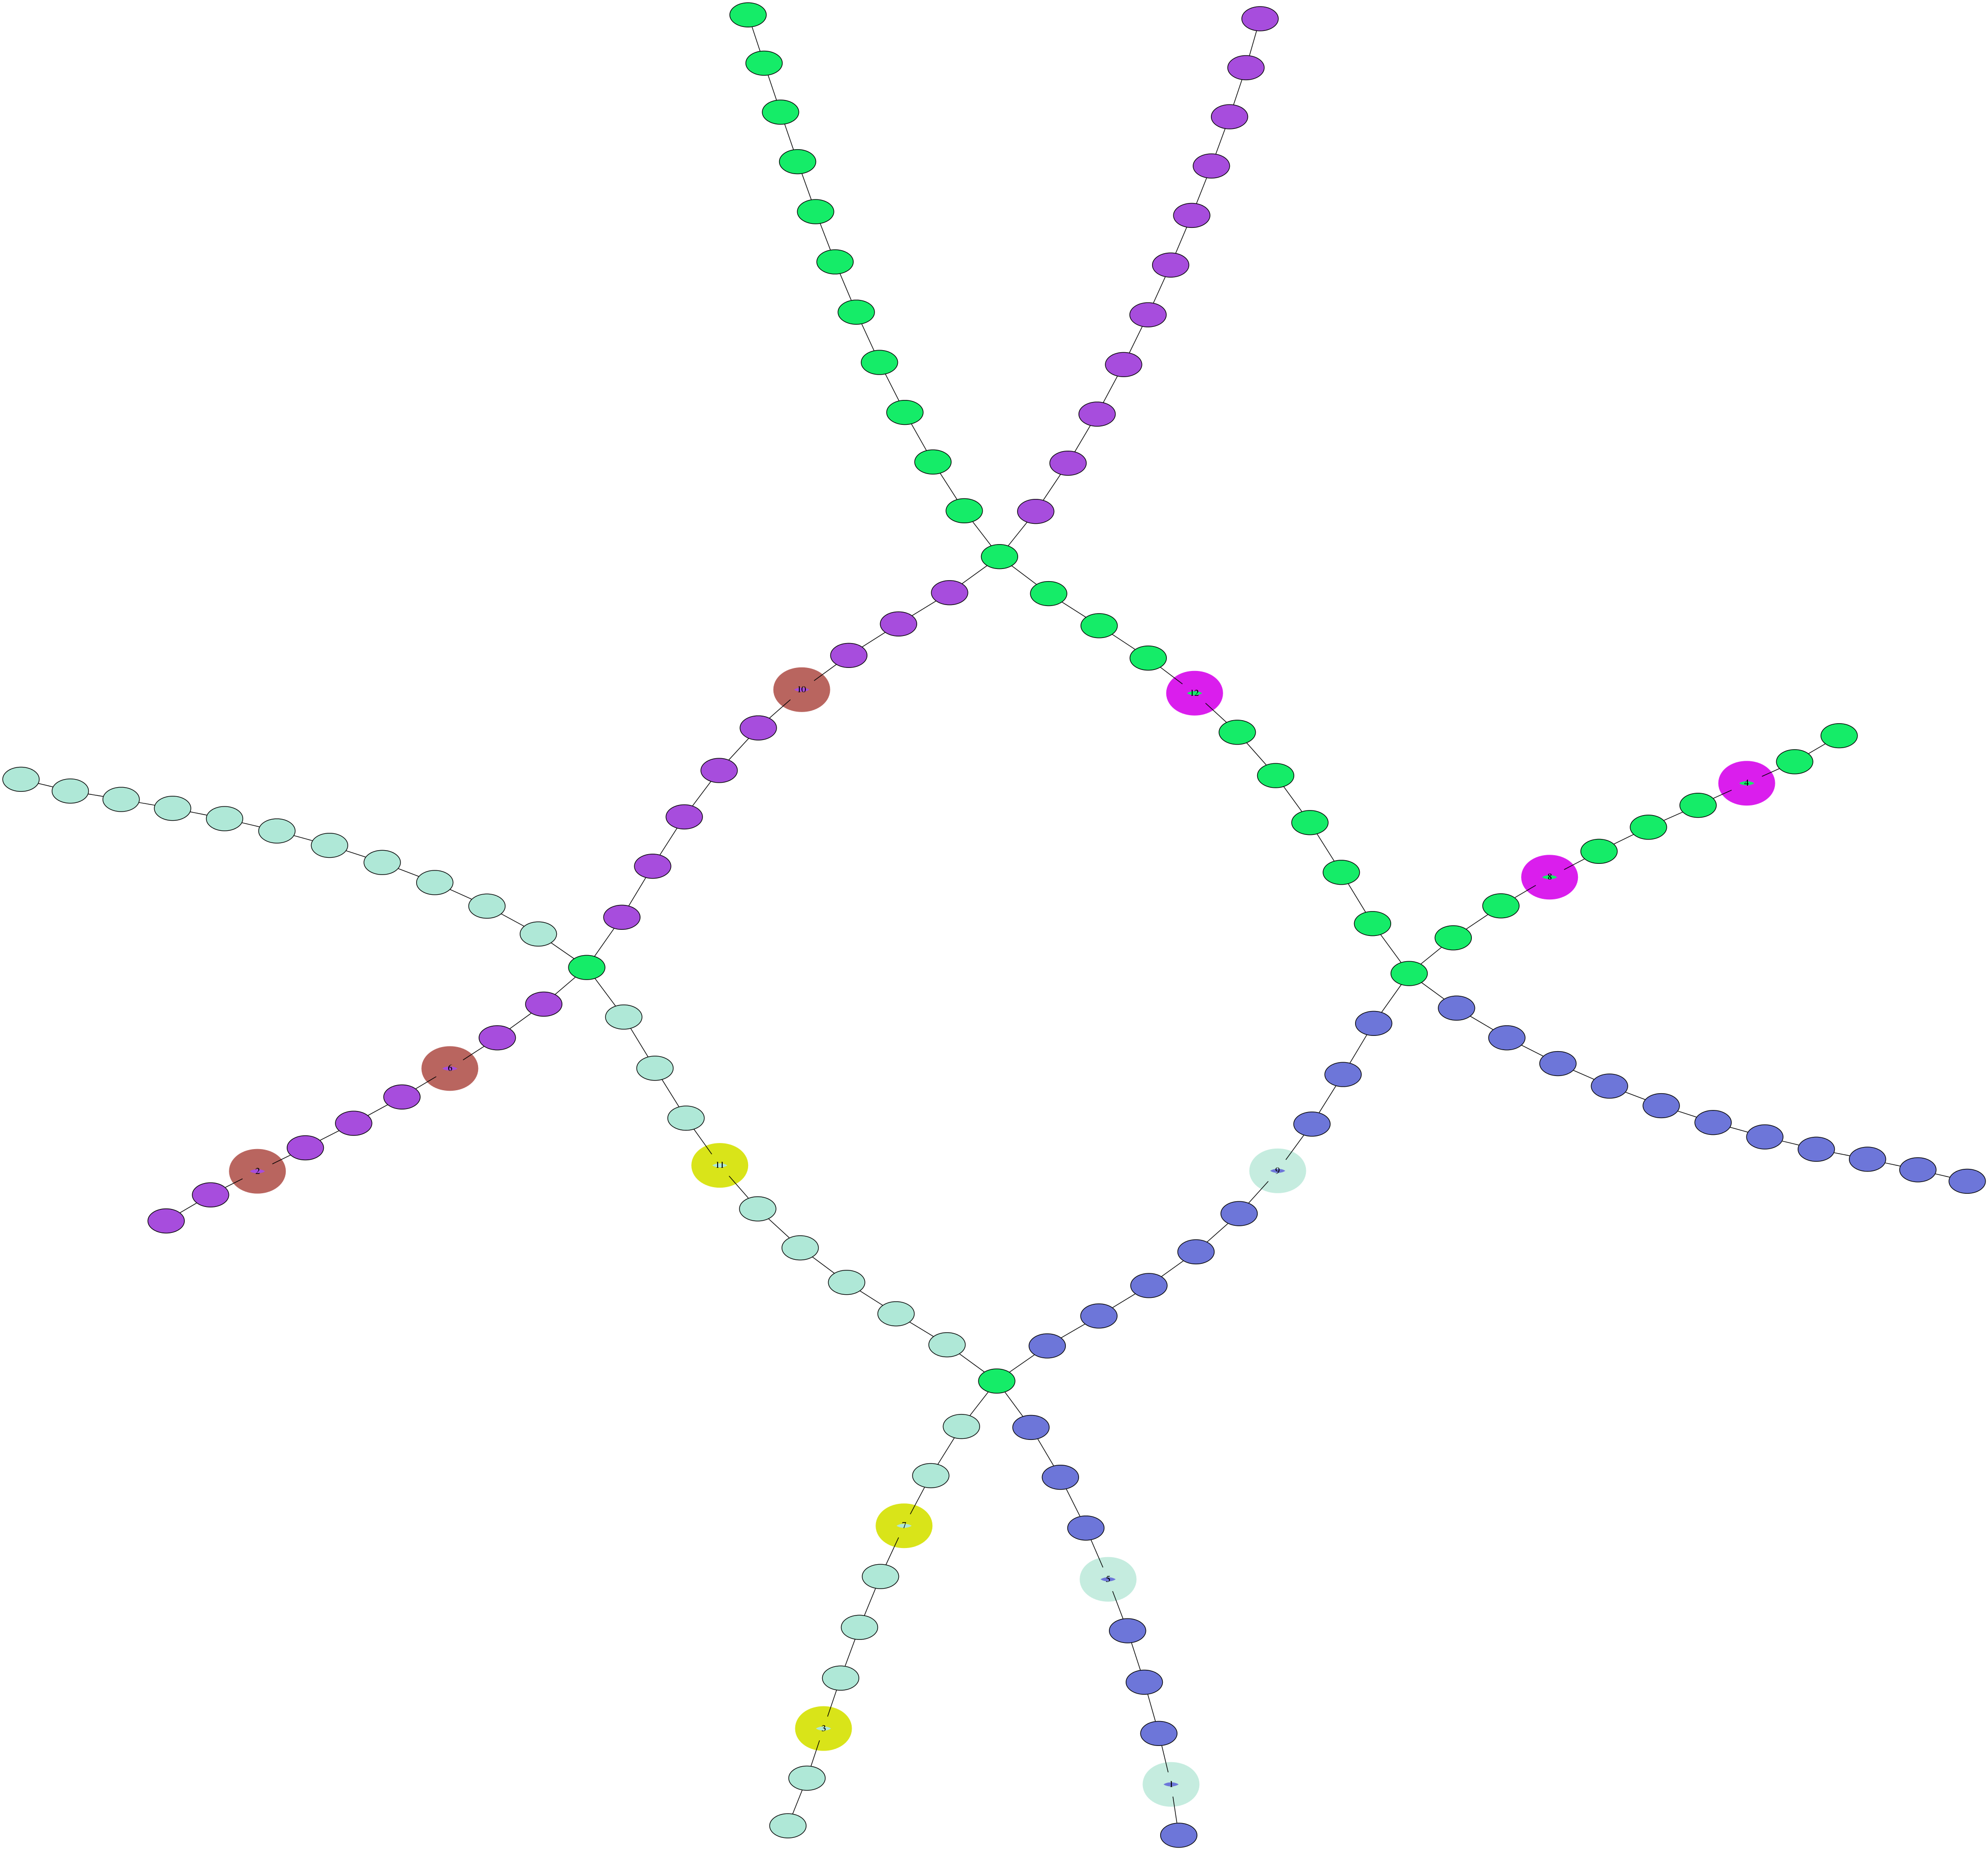
\includegraphics[width=1.0\textwidth]{2.png}
  \caption{2 krok czasowy}
  \label{2-traffic}
\end{figure}
\newpage
\begin{figure}
    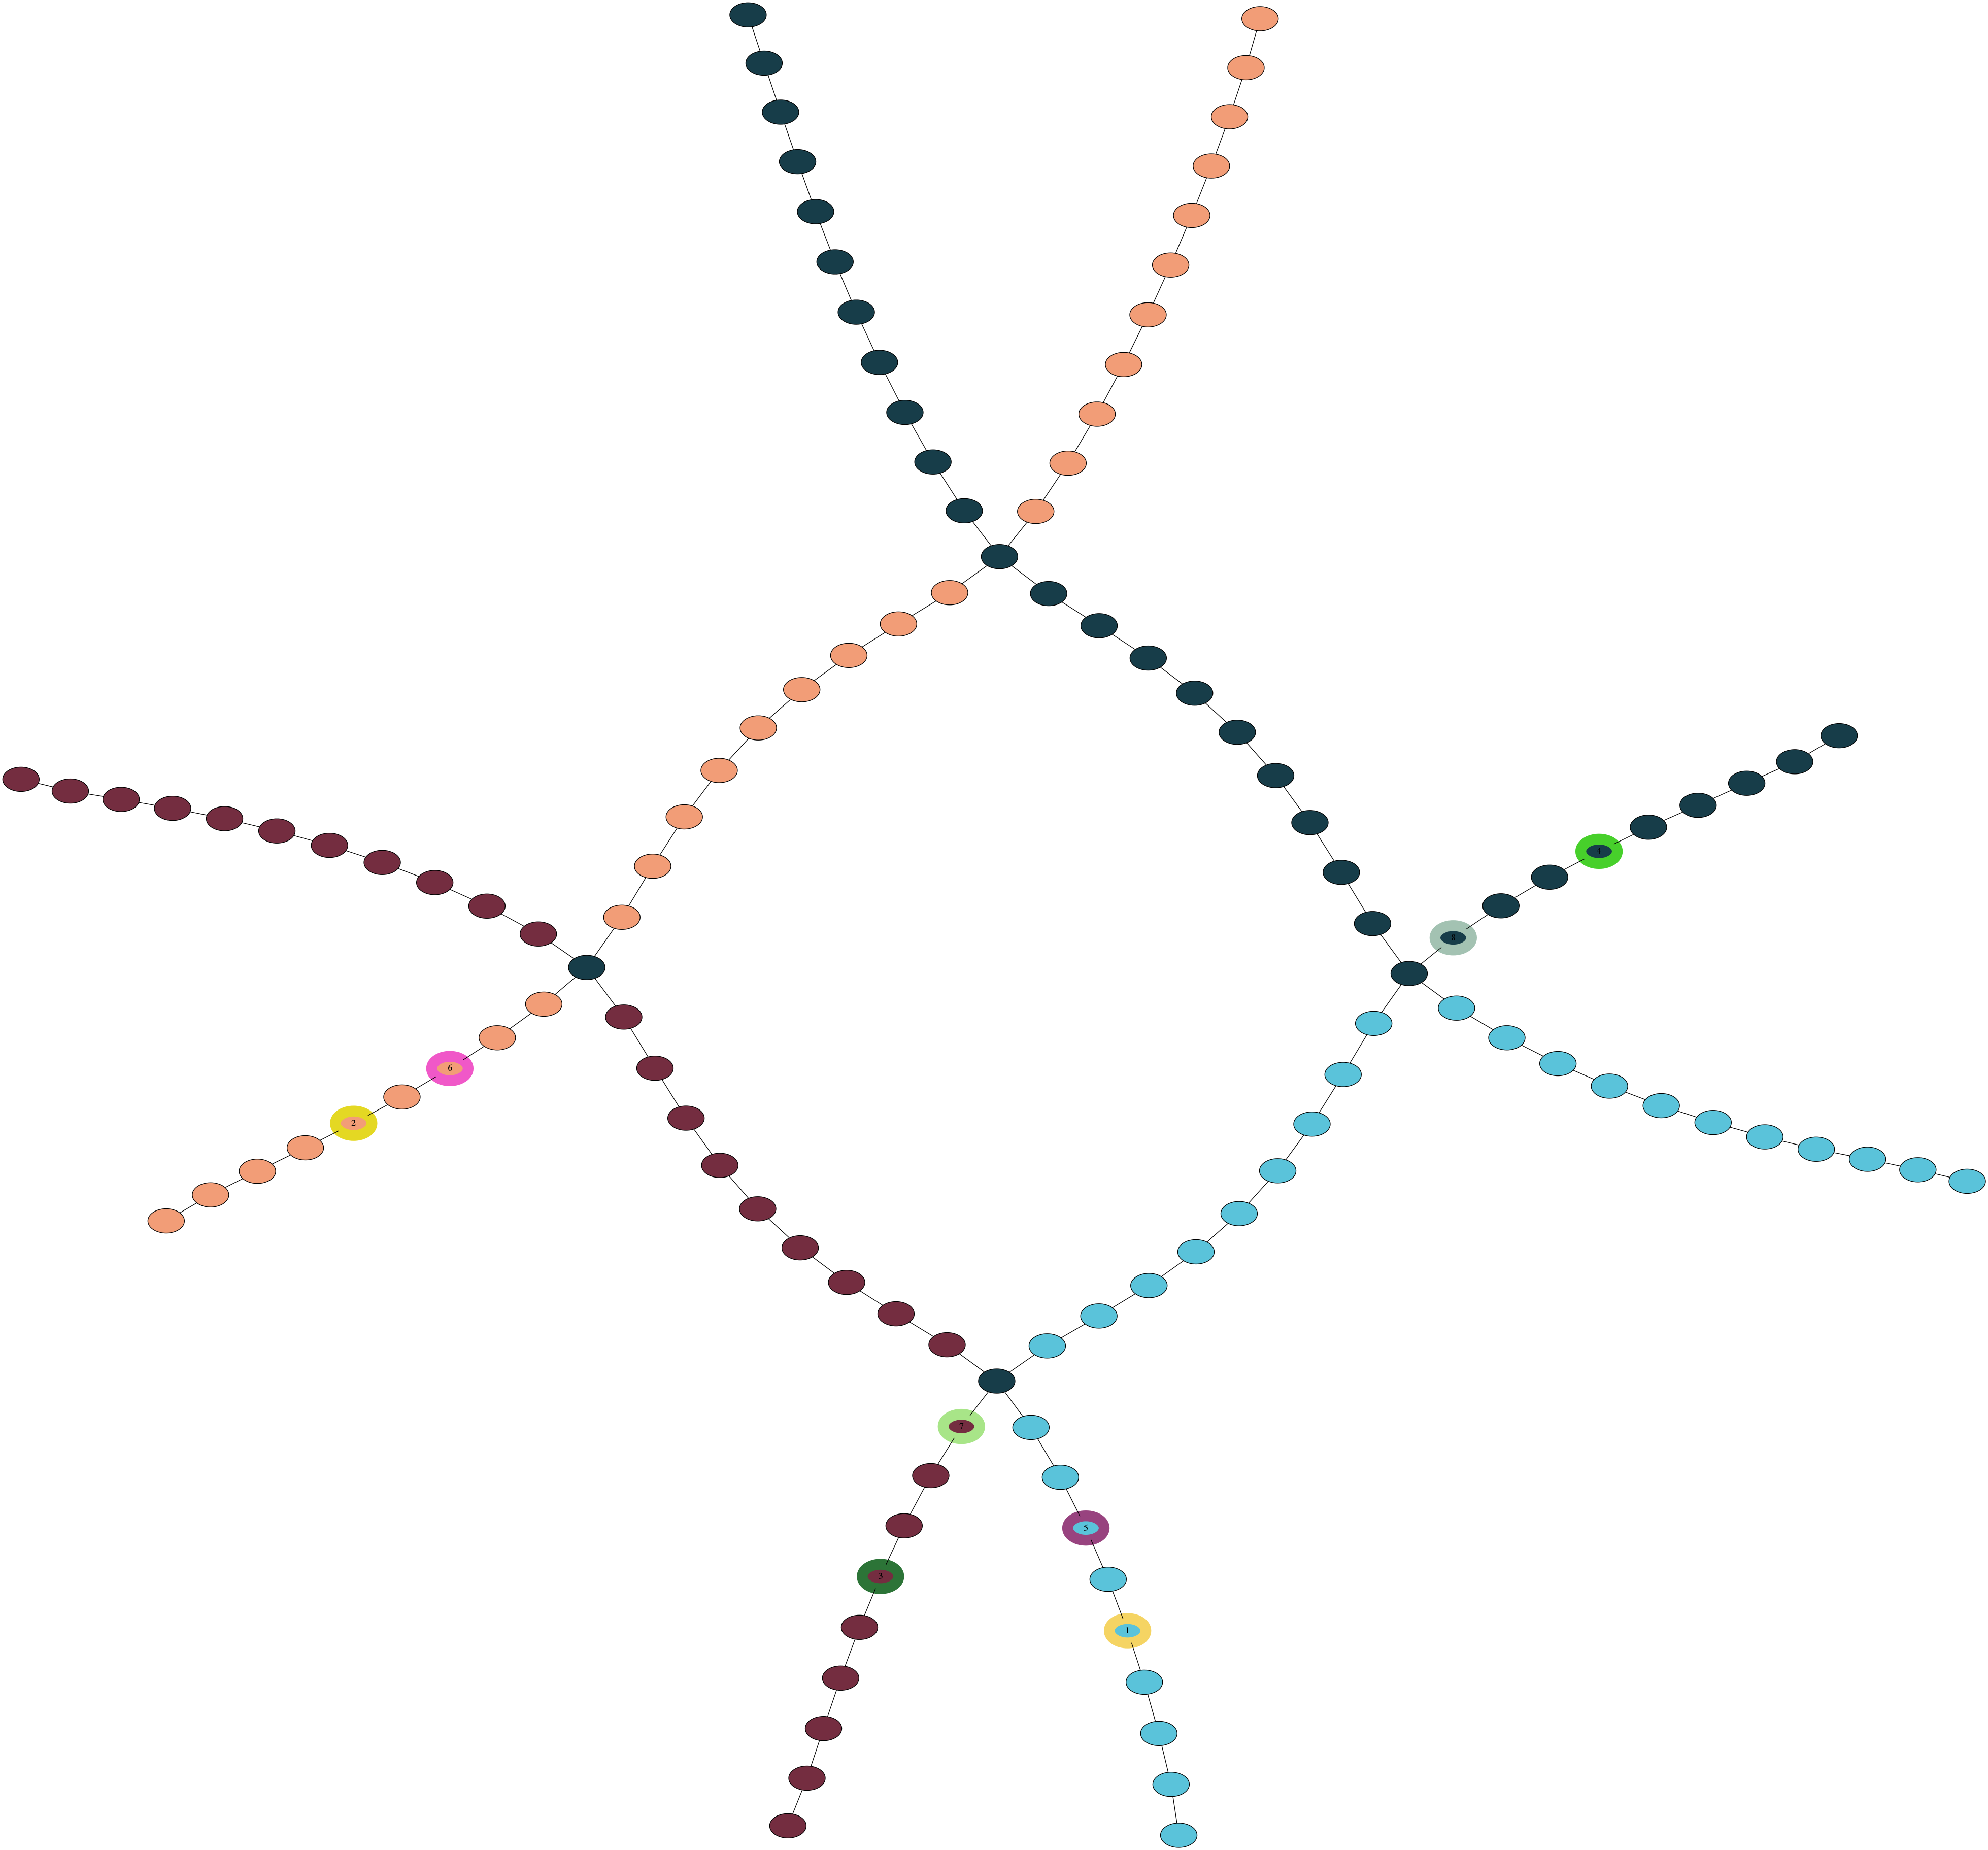
\includegraphics[width=1.0\textwidth]{3.png}
  \caption{3 krok czasowy}
  \label{3-traffic}
\end{figure}
\newpage
\begin{figure}
    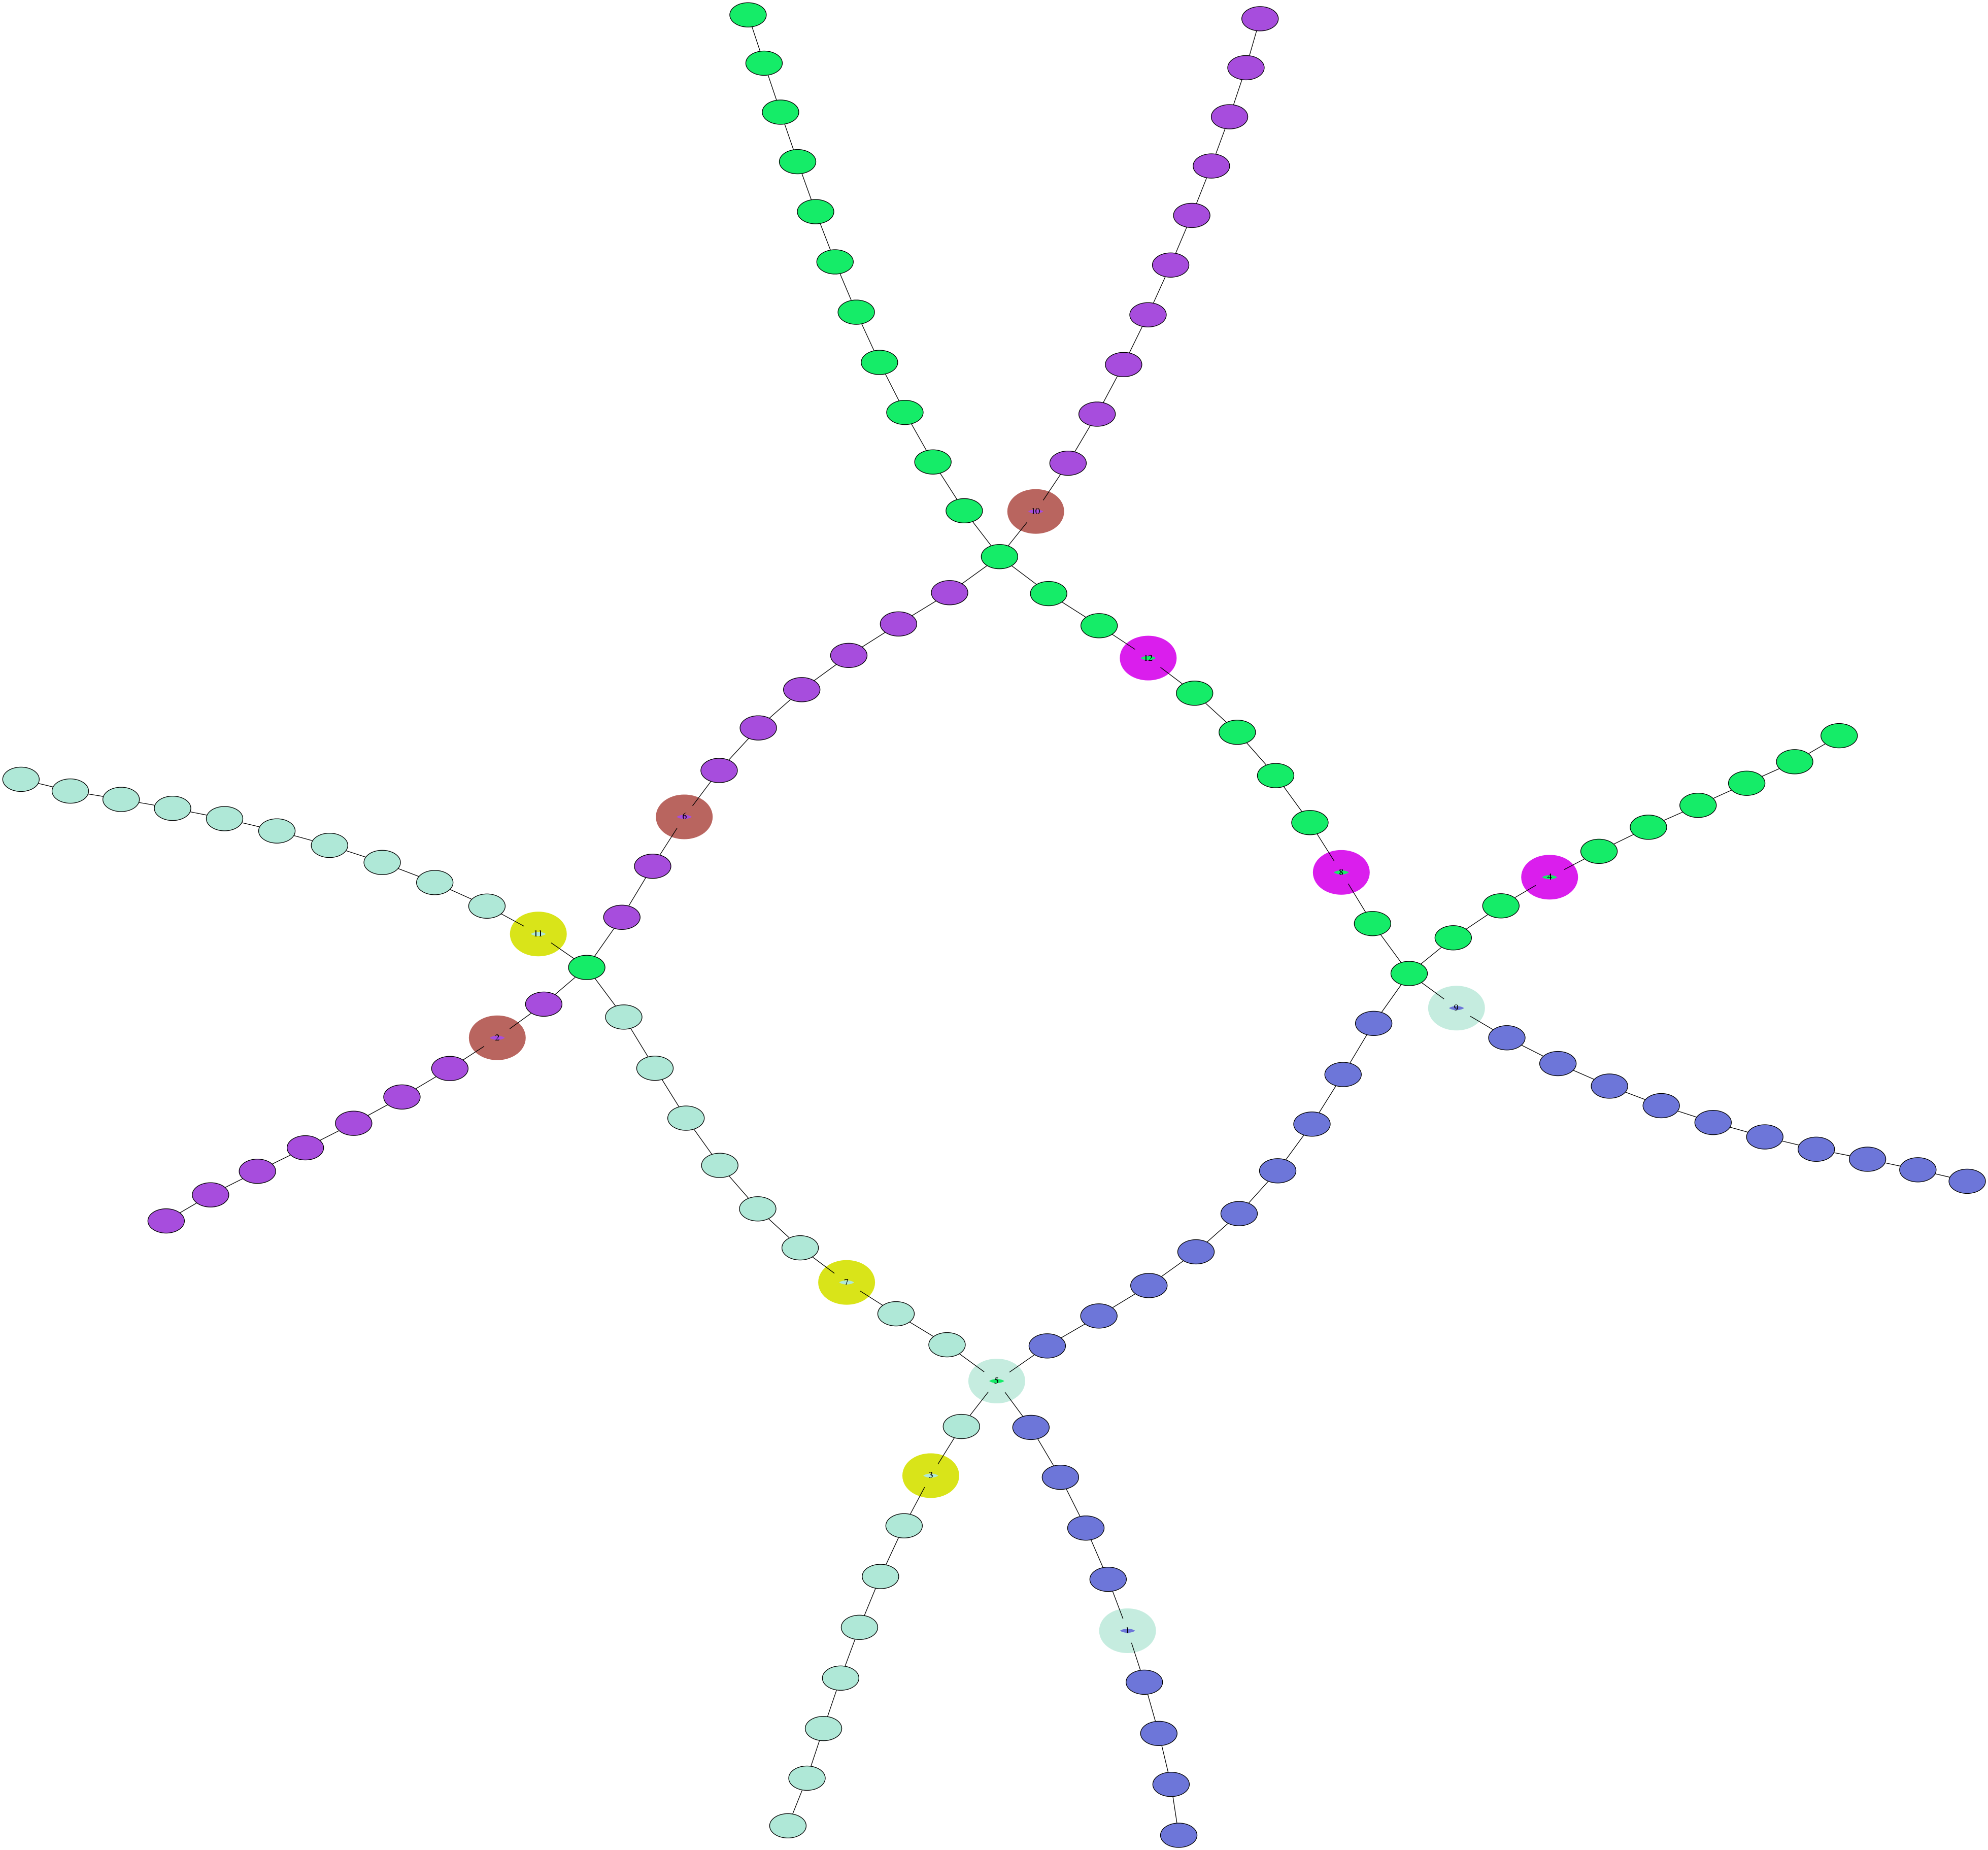
\includegraphics[width=1.0\textwidth]{4.png}
  \caption{4 krok czasowy}
  \label{4-traffic}
\end{figure}
\newpage
\begin{figure}
    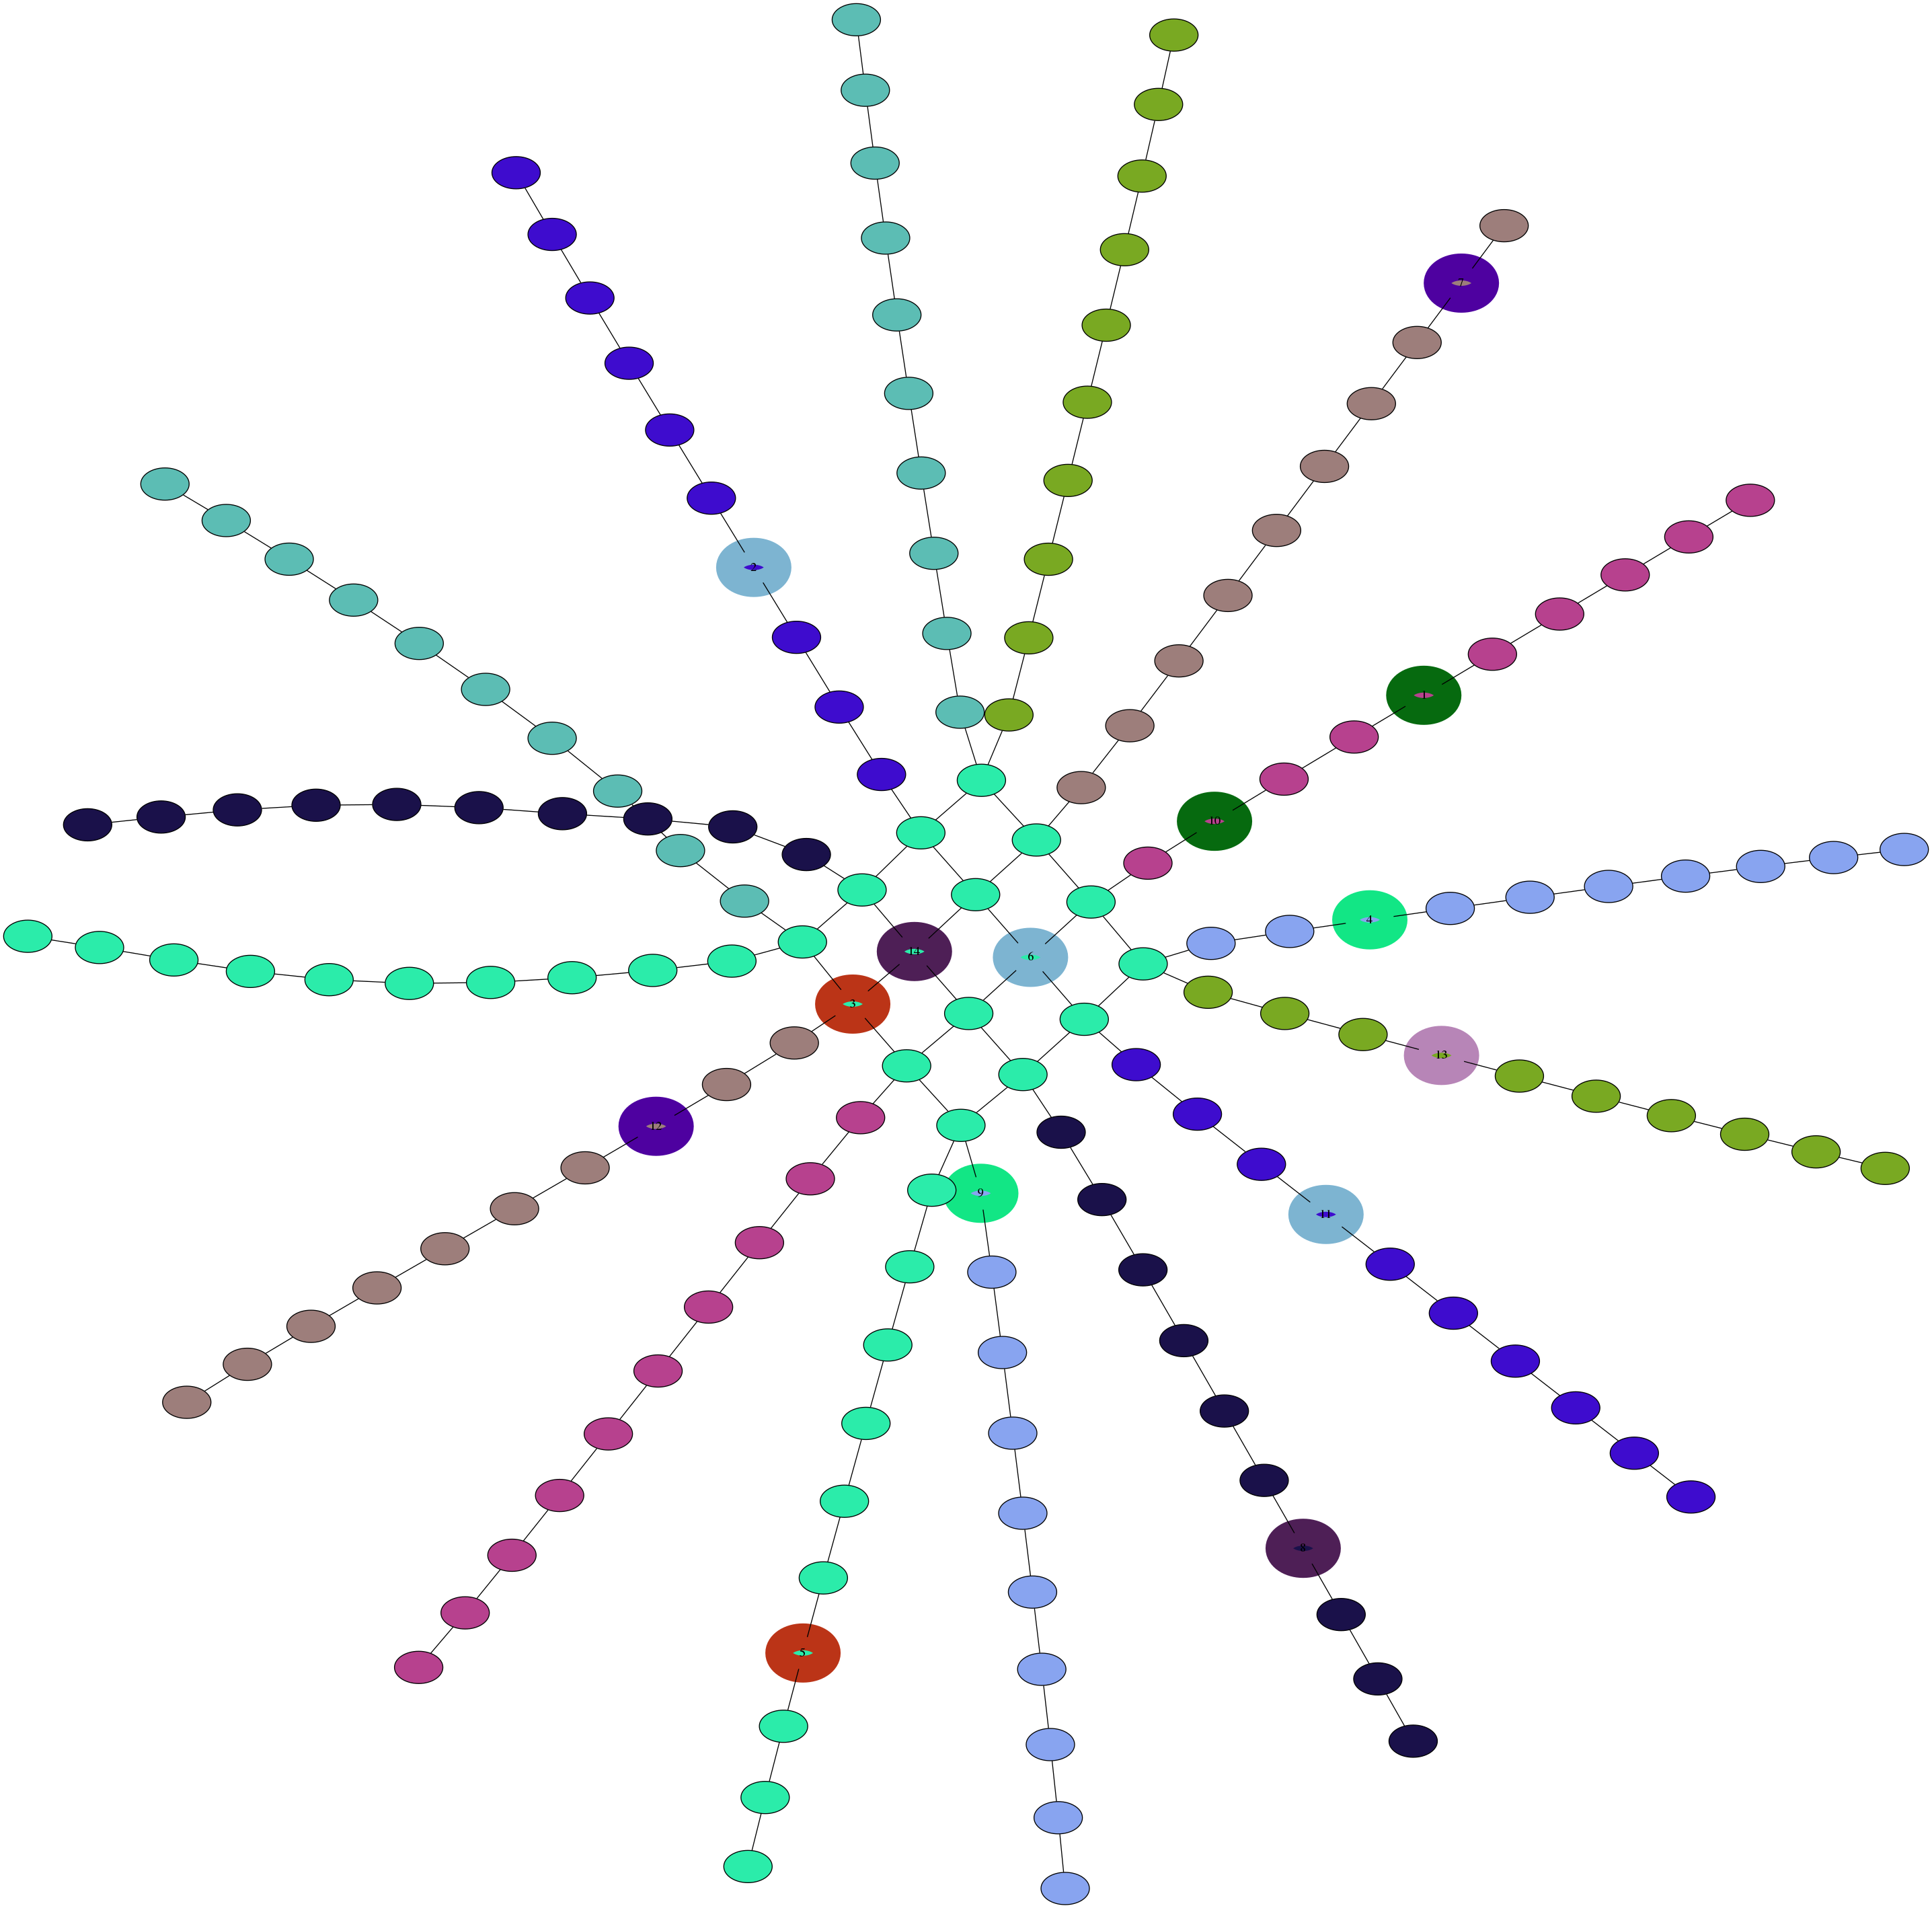
\includegraphics[width=1.0\textwidth]{5.png}
  \caption{5 krok czasowy}
  \label{5-traffic}
\end{figure}
\newpage
\begin{figure}
    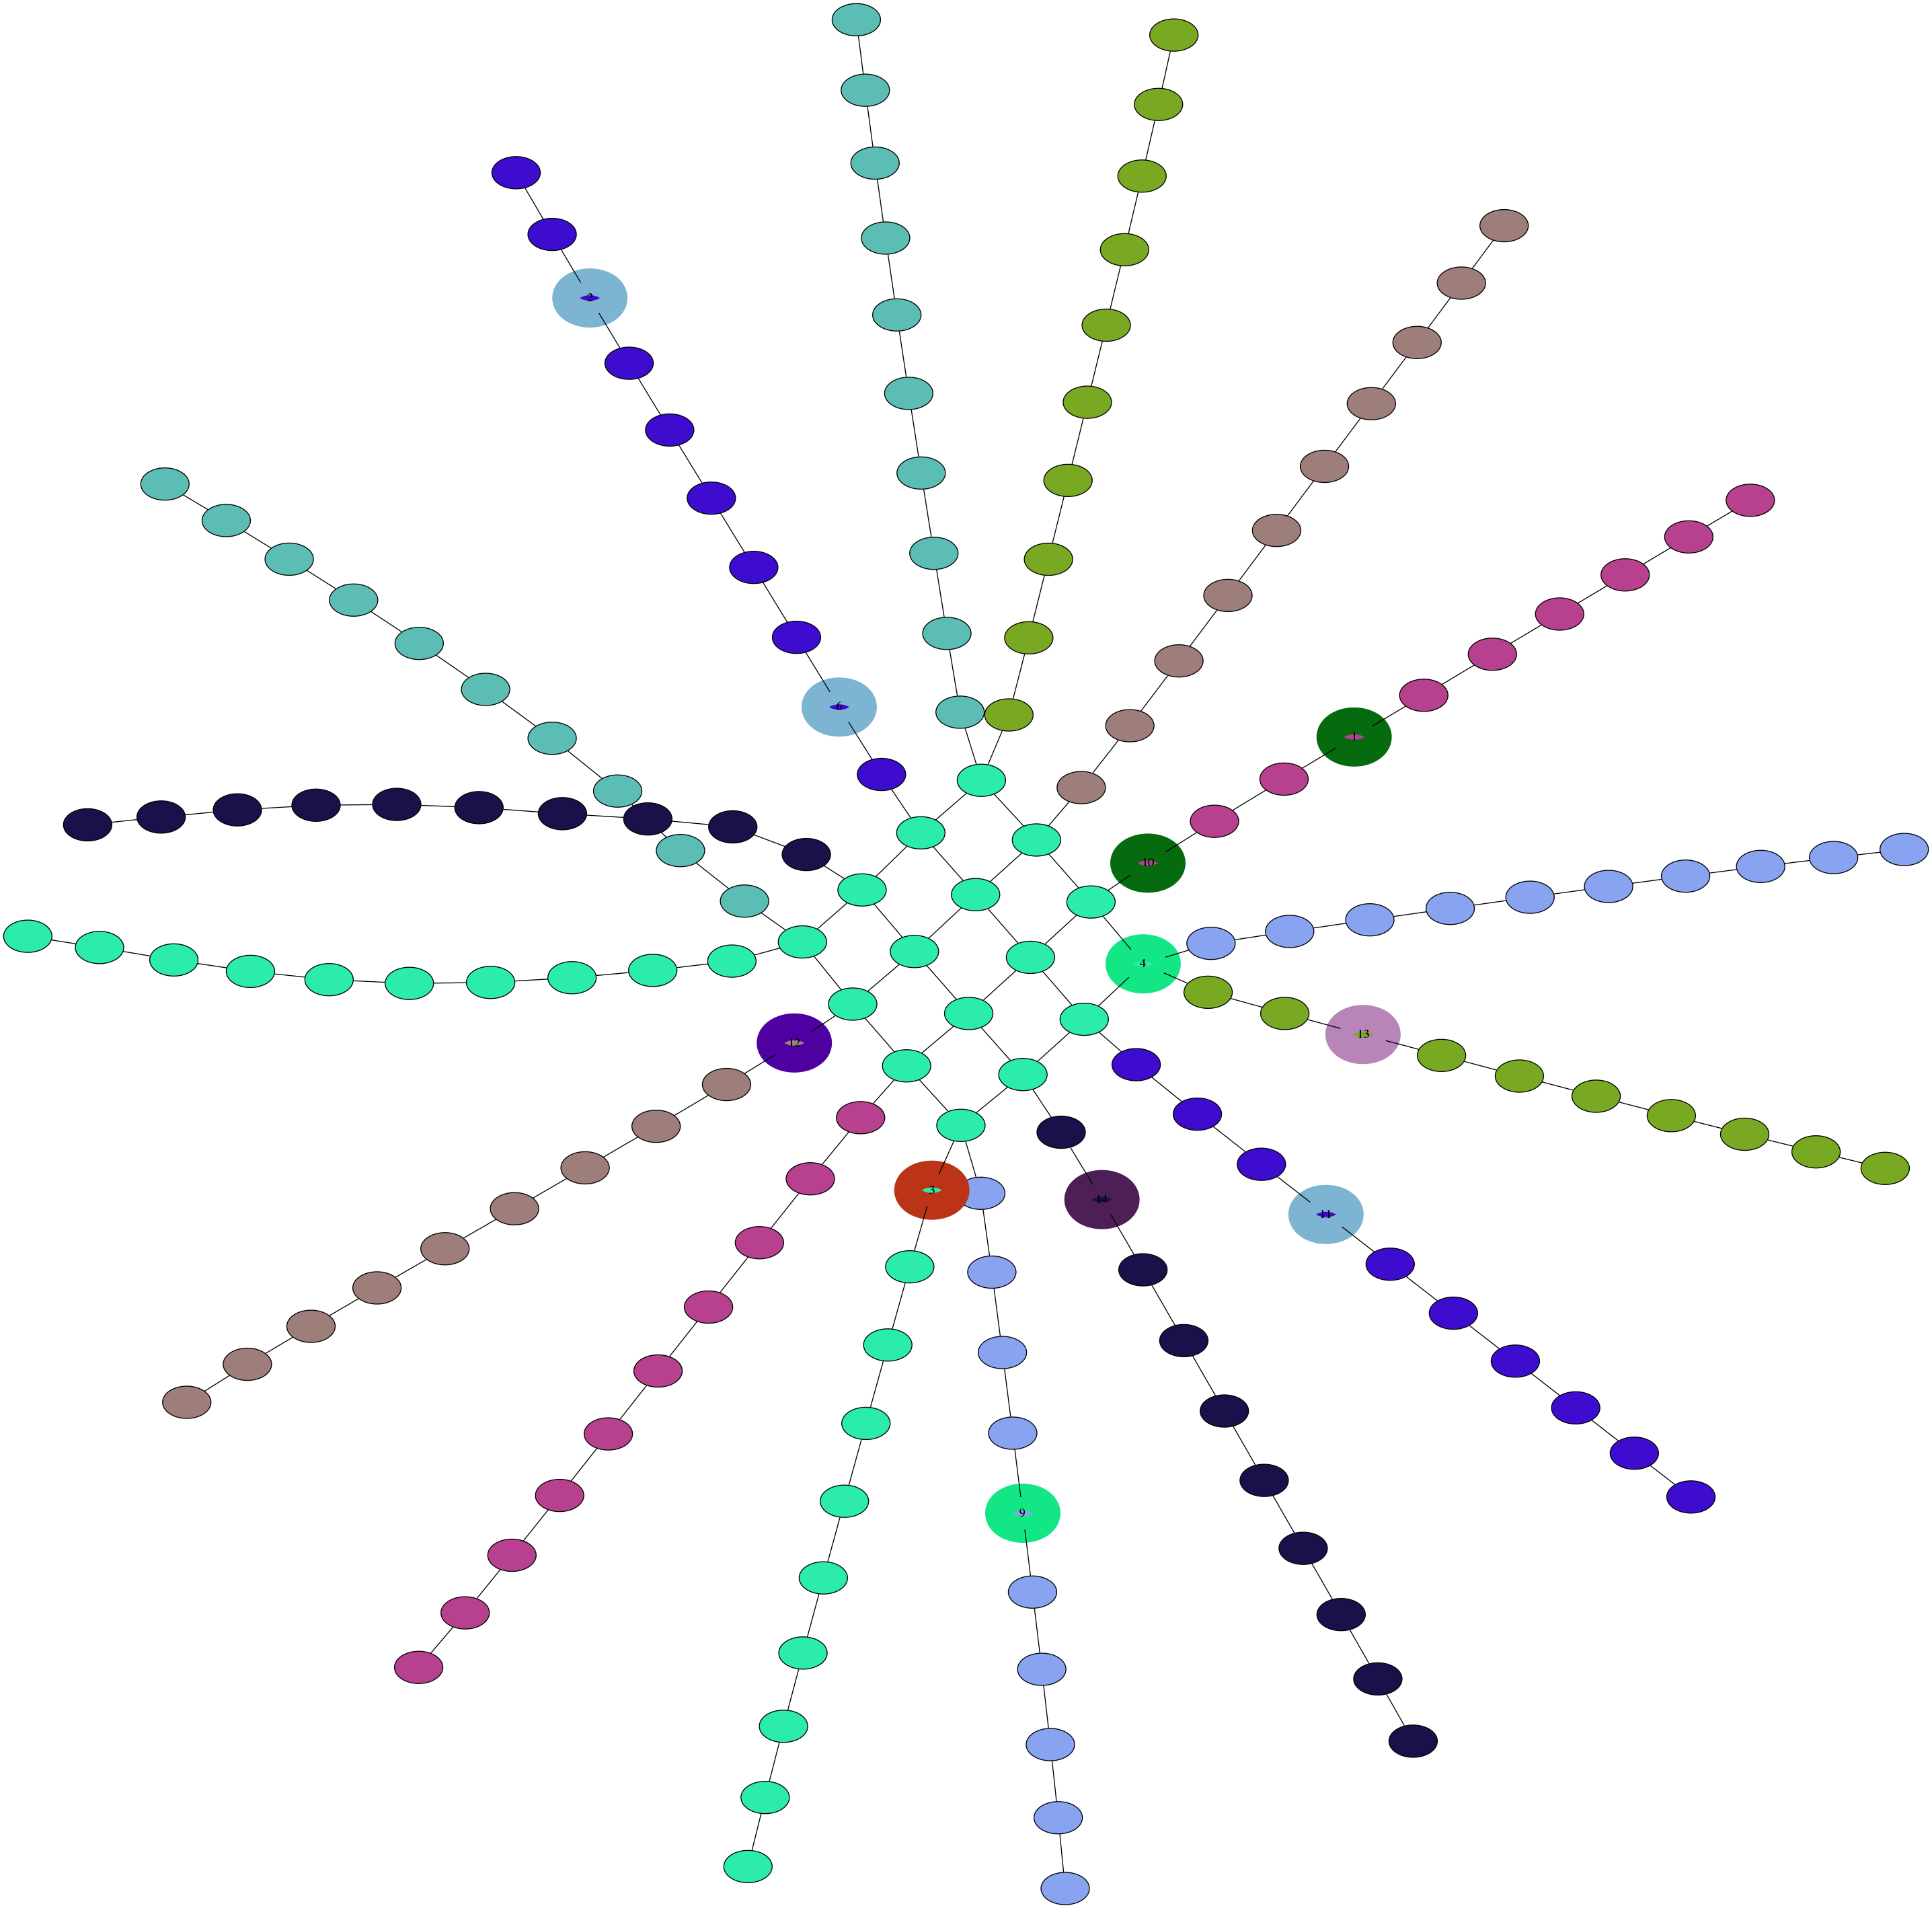
\includegraphics[width=1.0\textwidth]{6.png}
  \caption{6 krok czasowy}
  \label{6-traffic}
\end{figure}
\newpage
\begin{figure}
    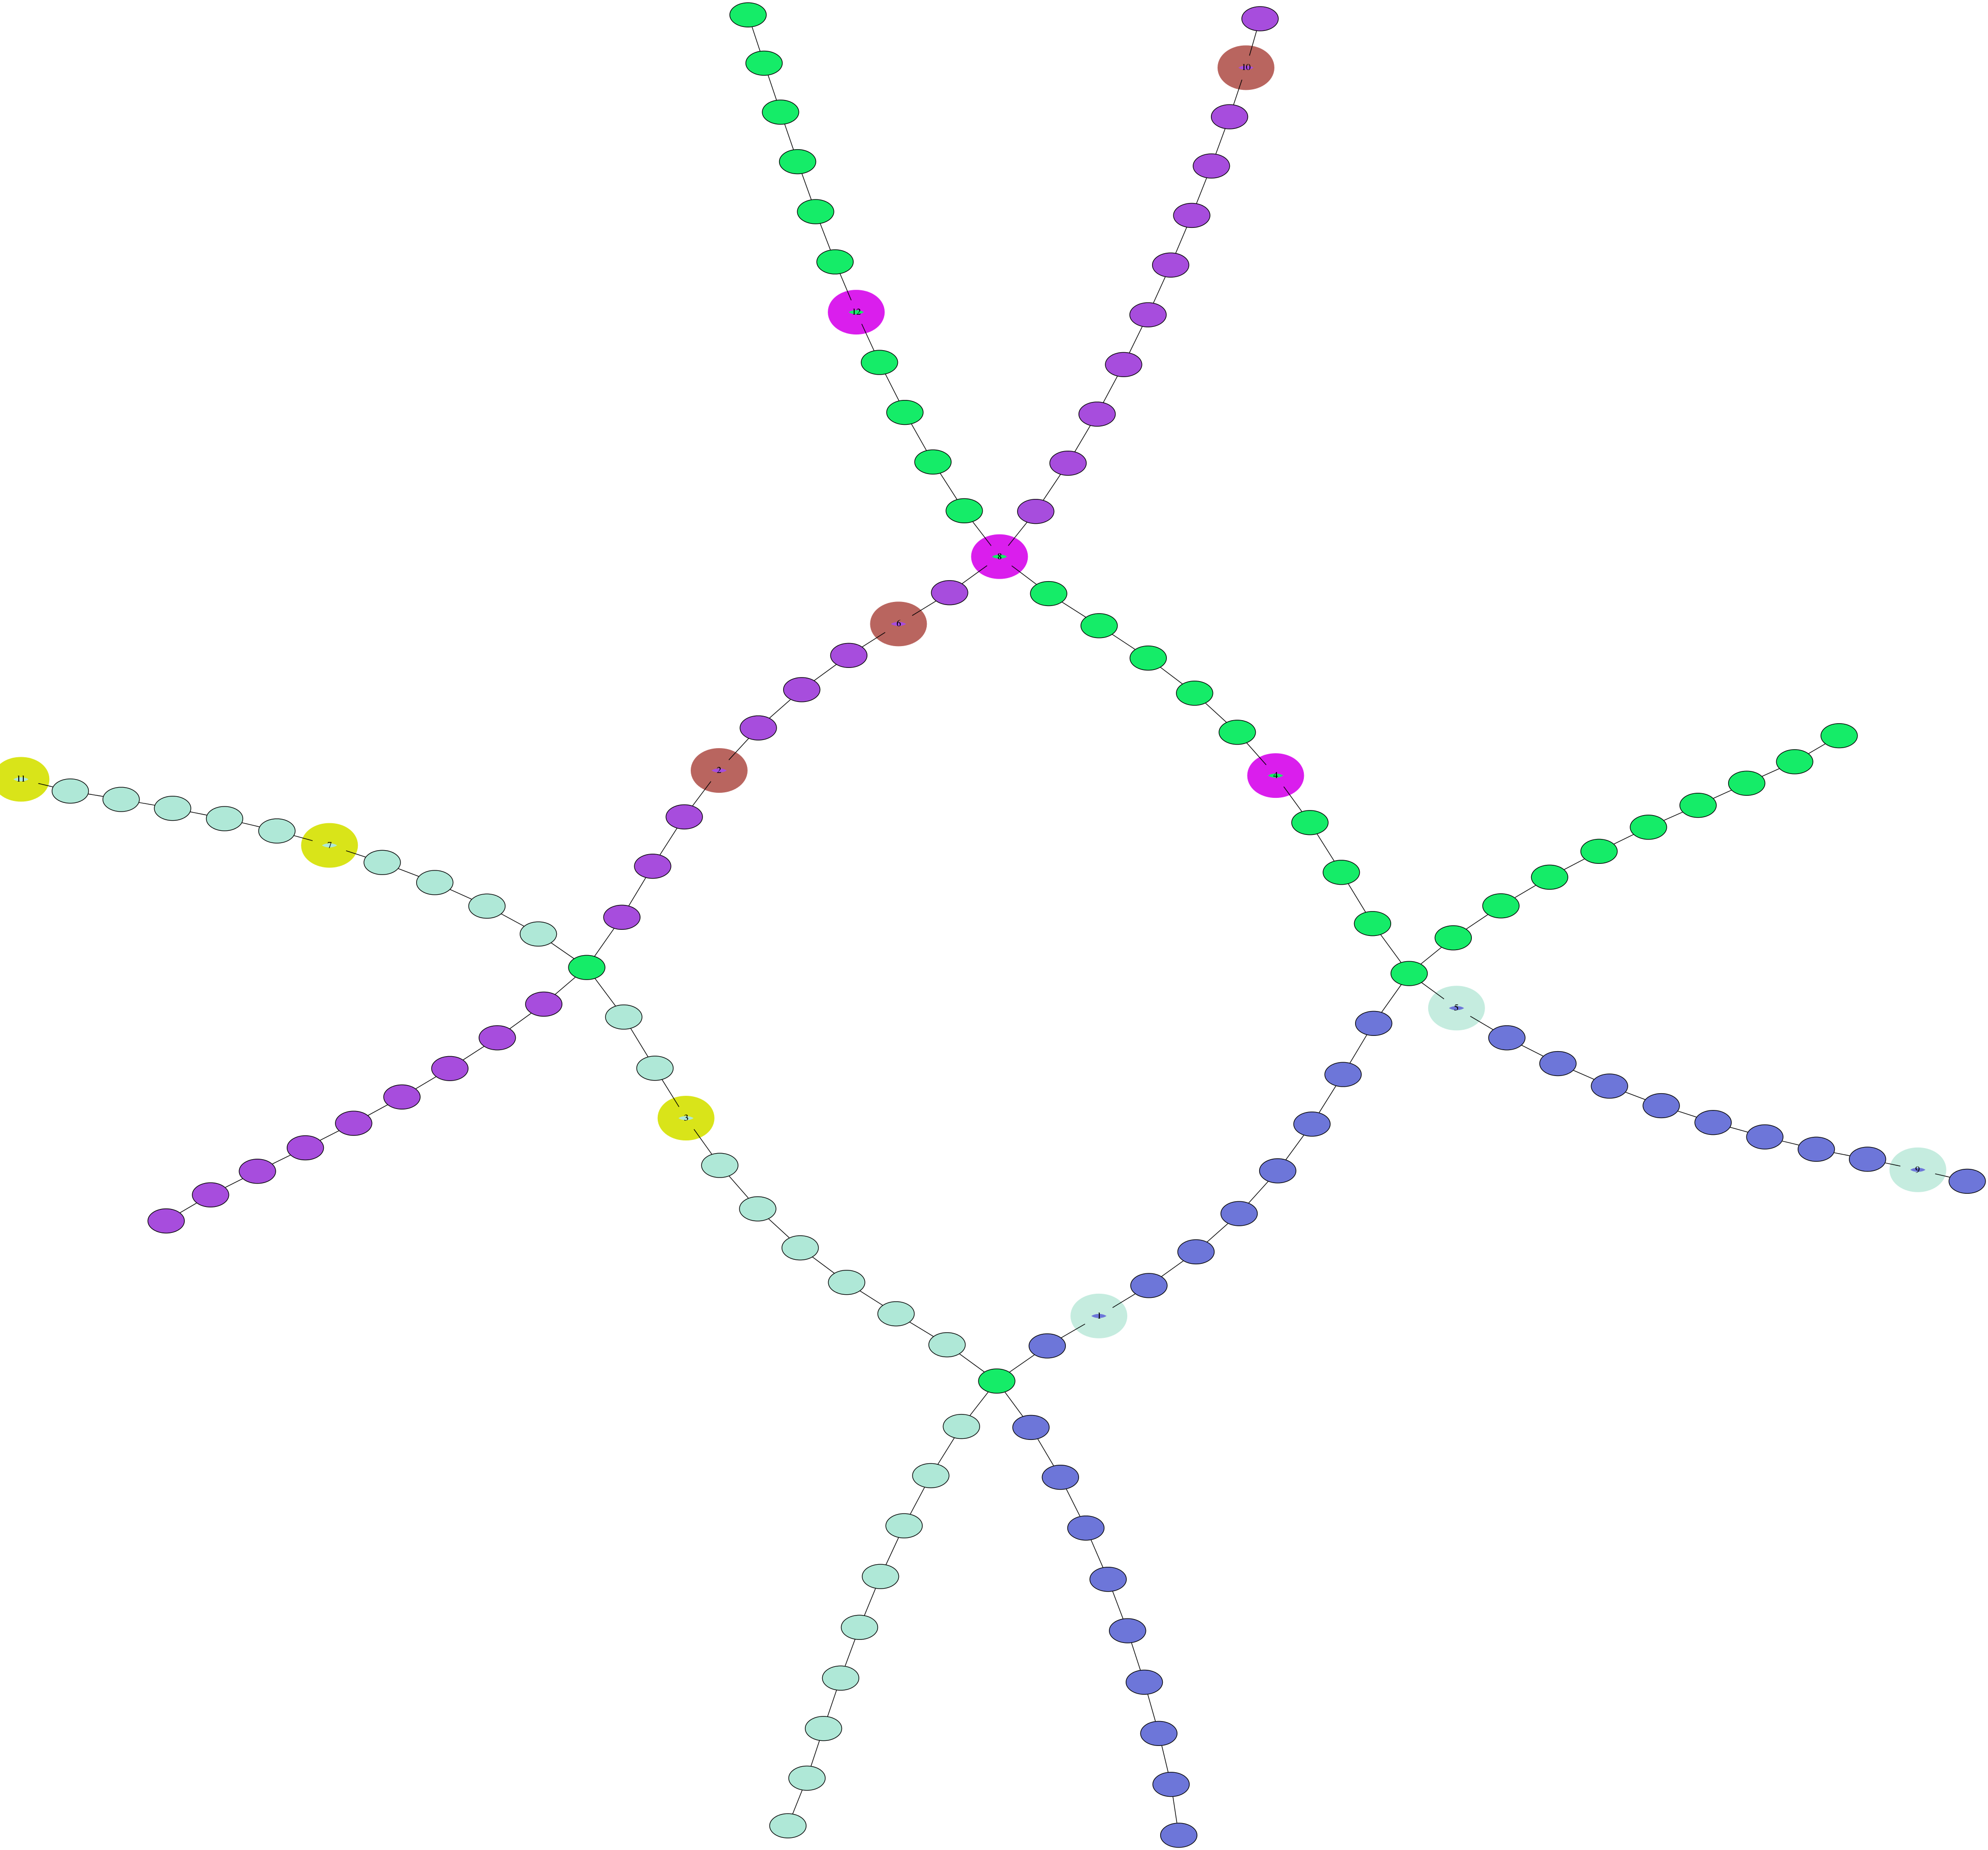
\includegraphics[width=1.0\textwidth]{7.png}
  \caption{7 krok czasowy}
  \label{7-traffic}
\end{figure}
\newpage
\begin{figure}
    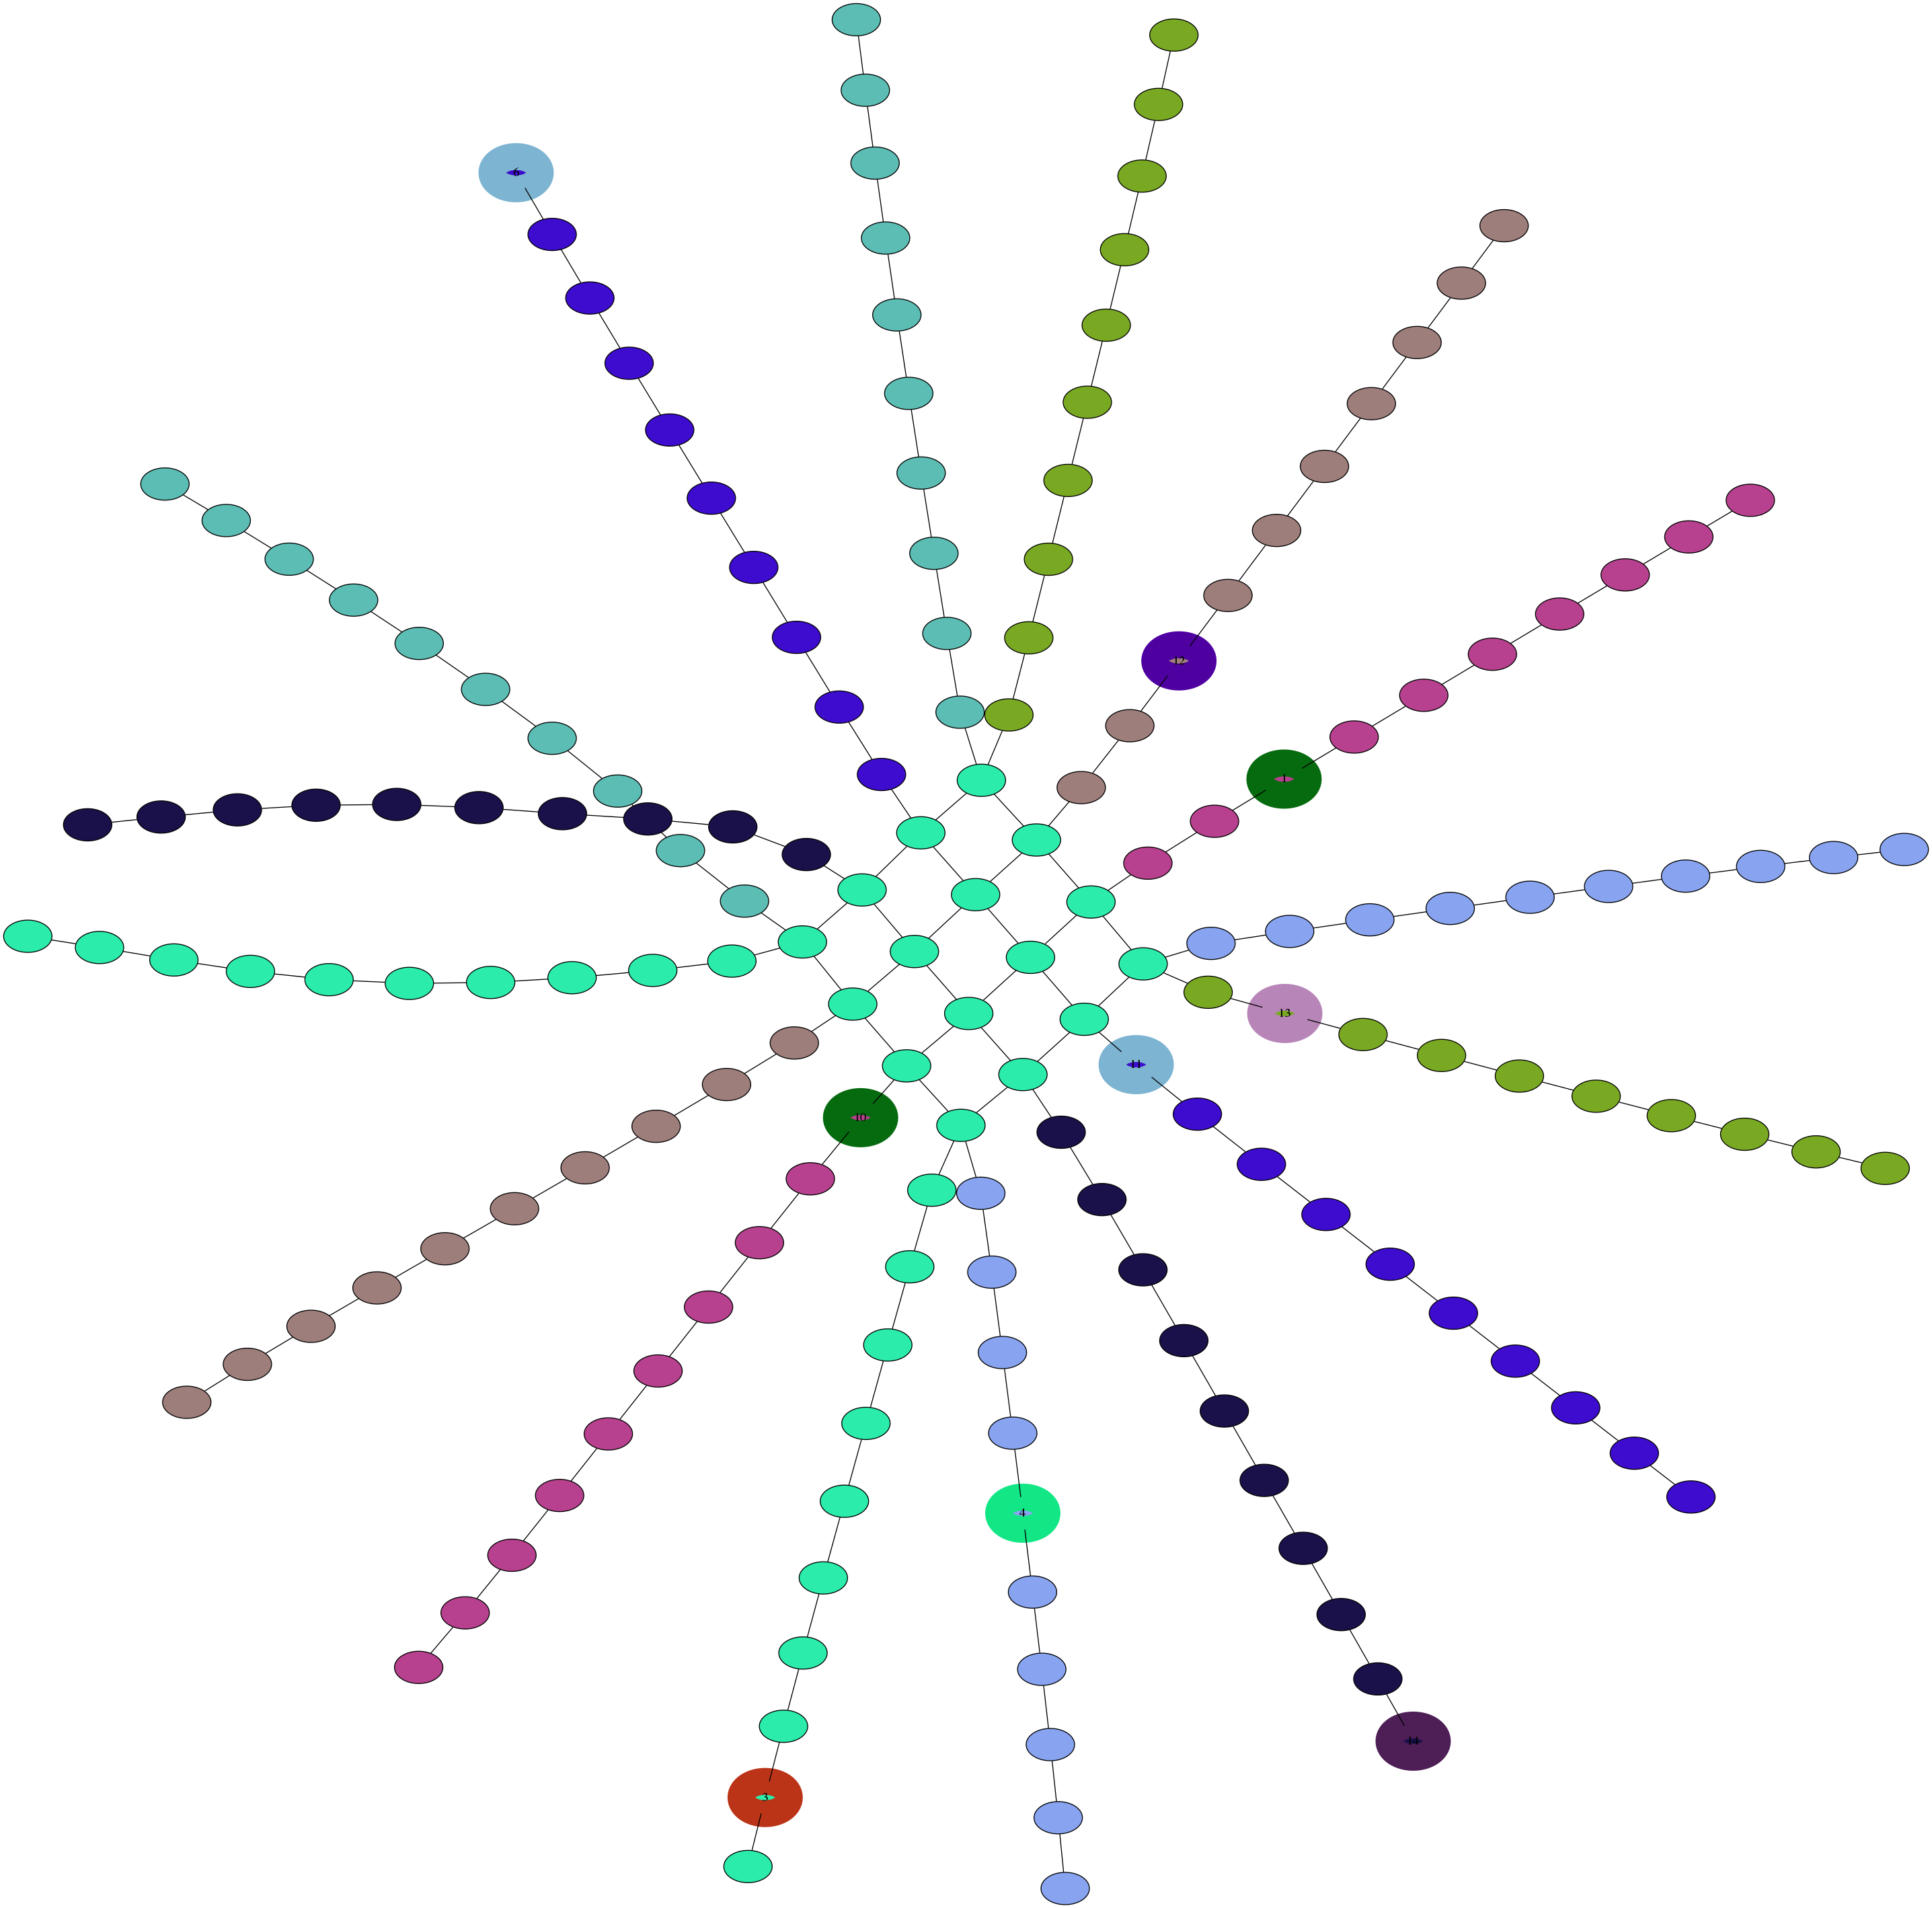
\includegraphics[width=1.0\textwidth]{8.png}
  \caption{8 krok czasowy}
  \label{8-traffic}
\end{figure}
\newpage
\begin{figure}
    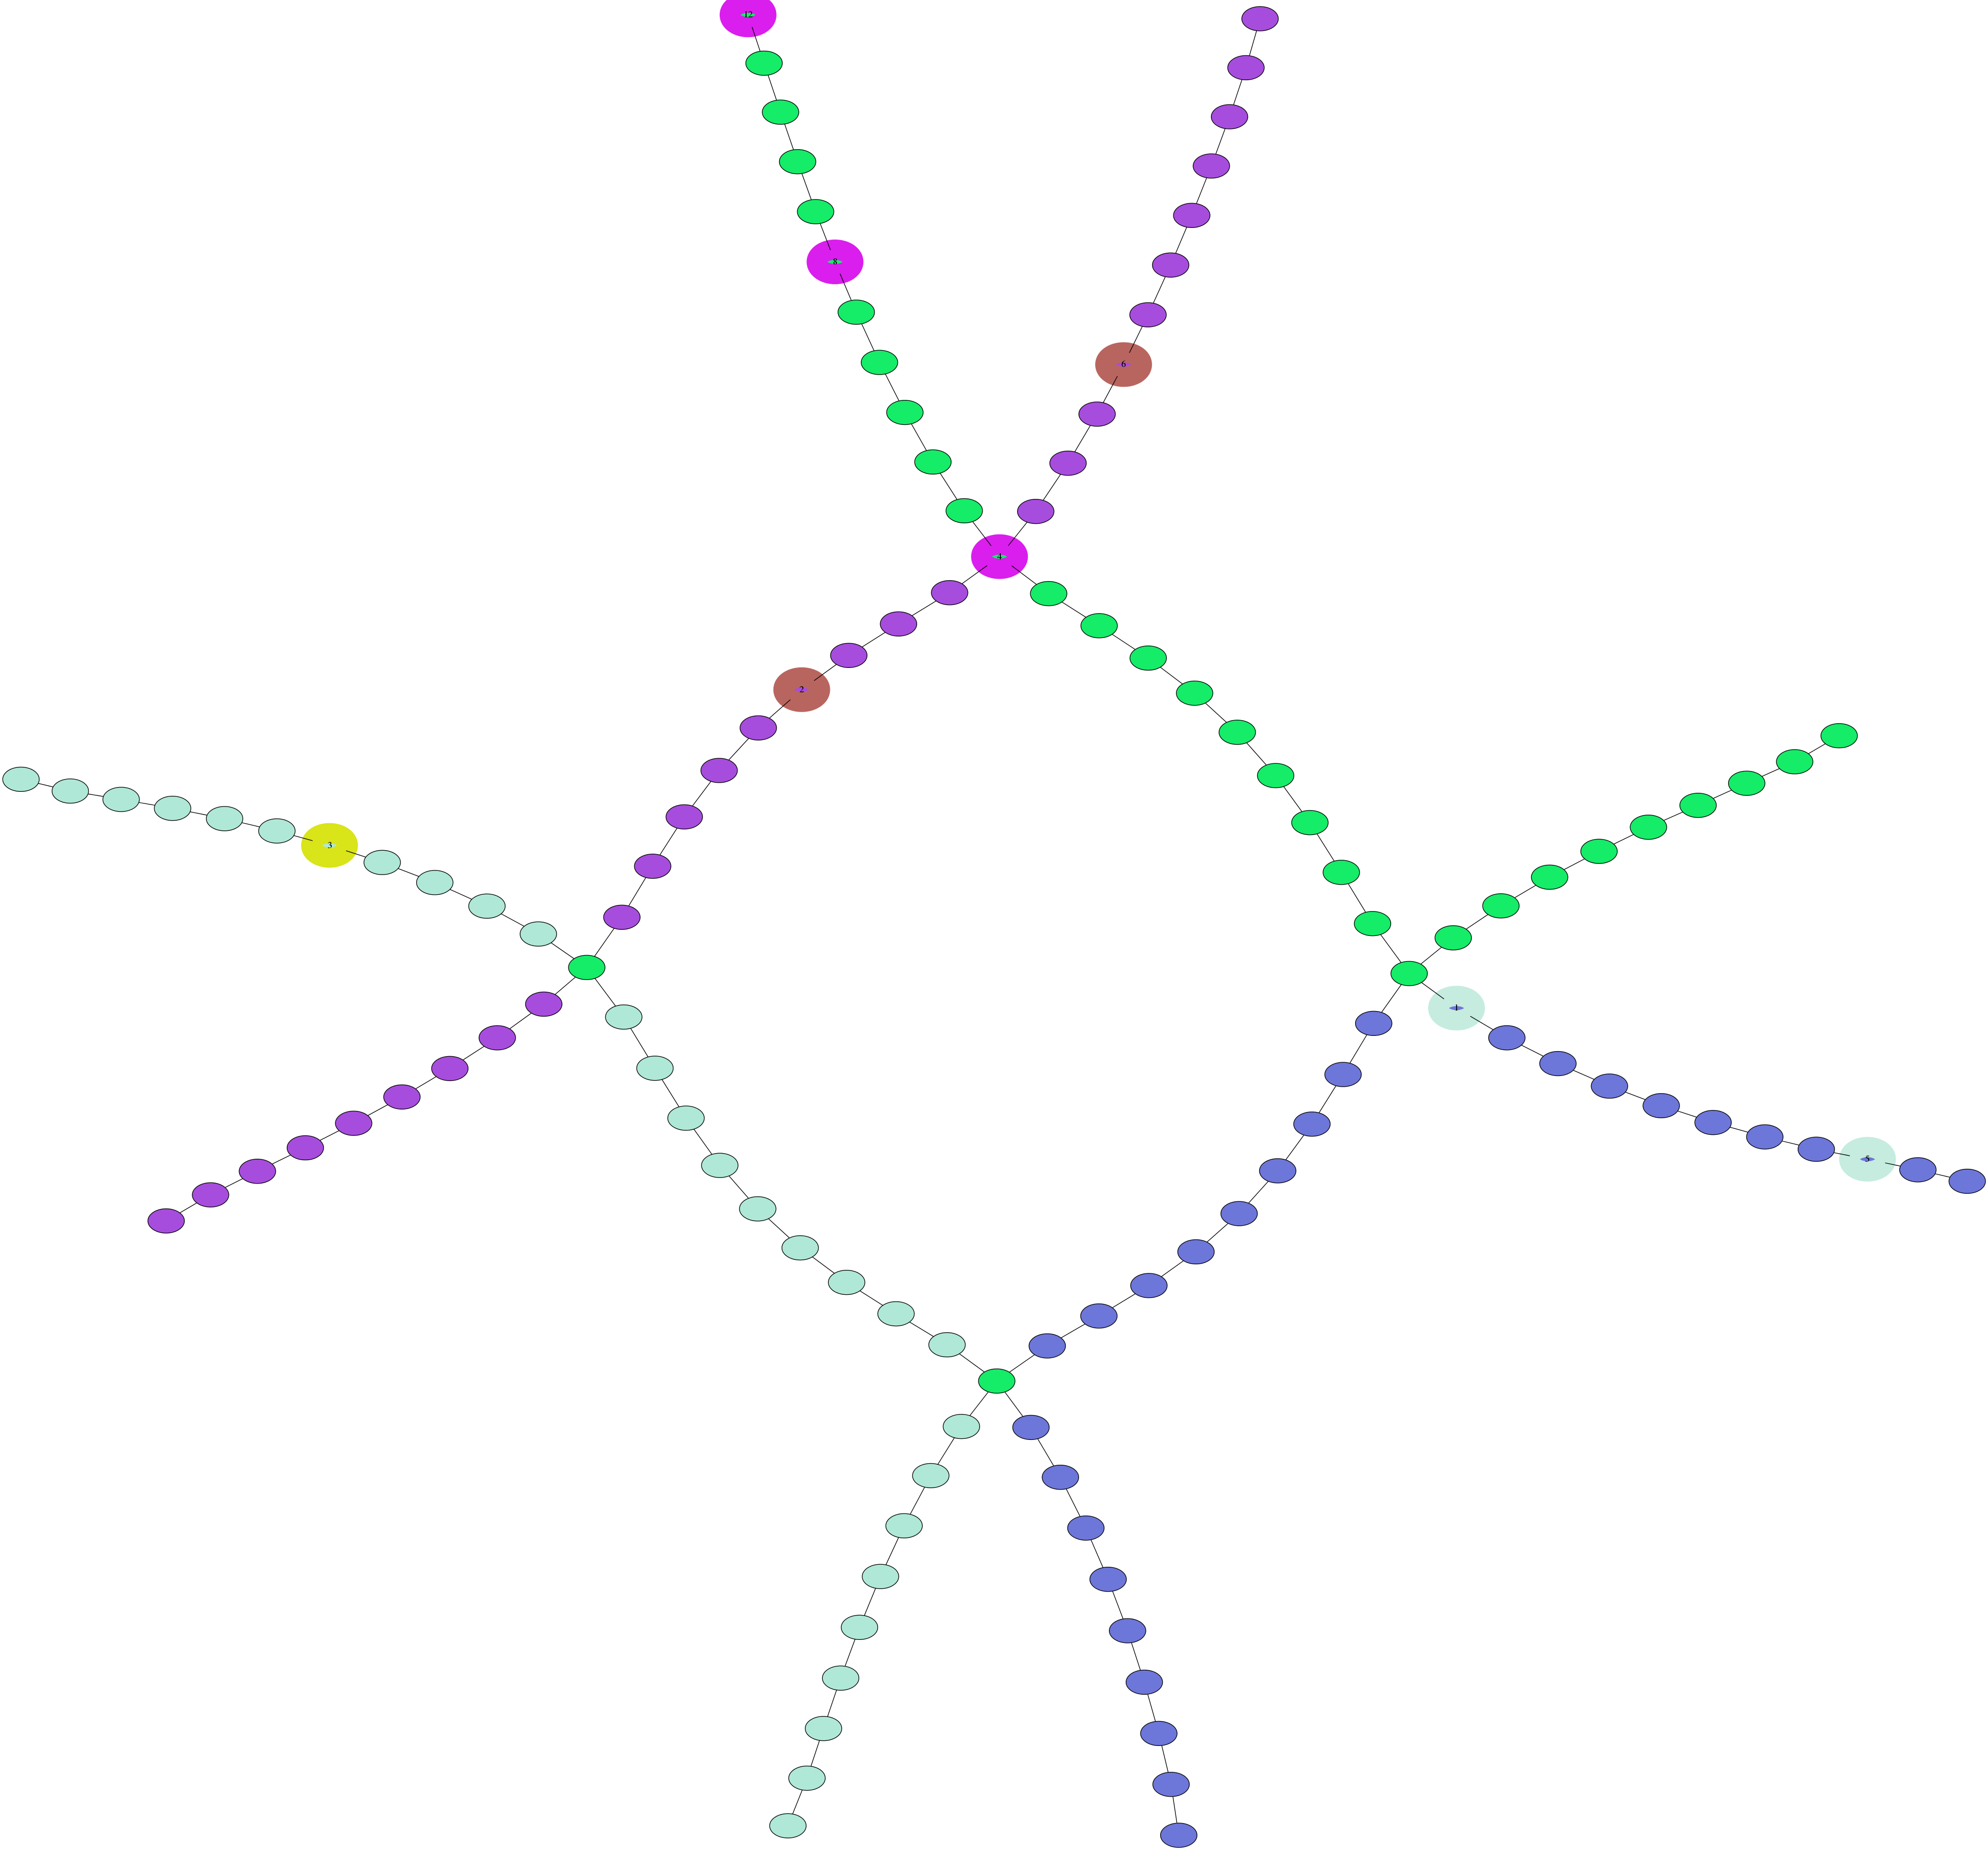
\includegraphics[width=1.0\textwidth]{9.png}
  \caption{9 krok czasowy}
  \label{9-traffic}
\end{figure}
\newpage
\begin{figure}
    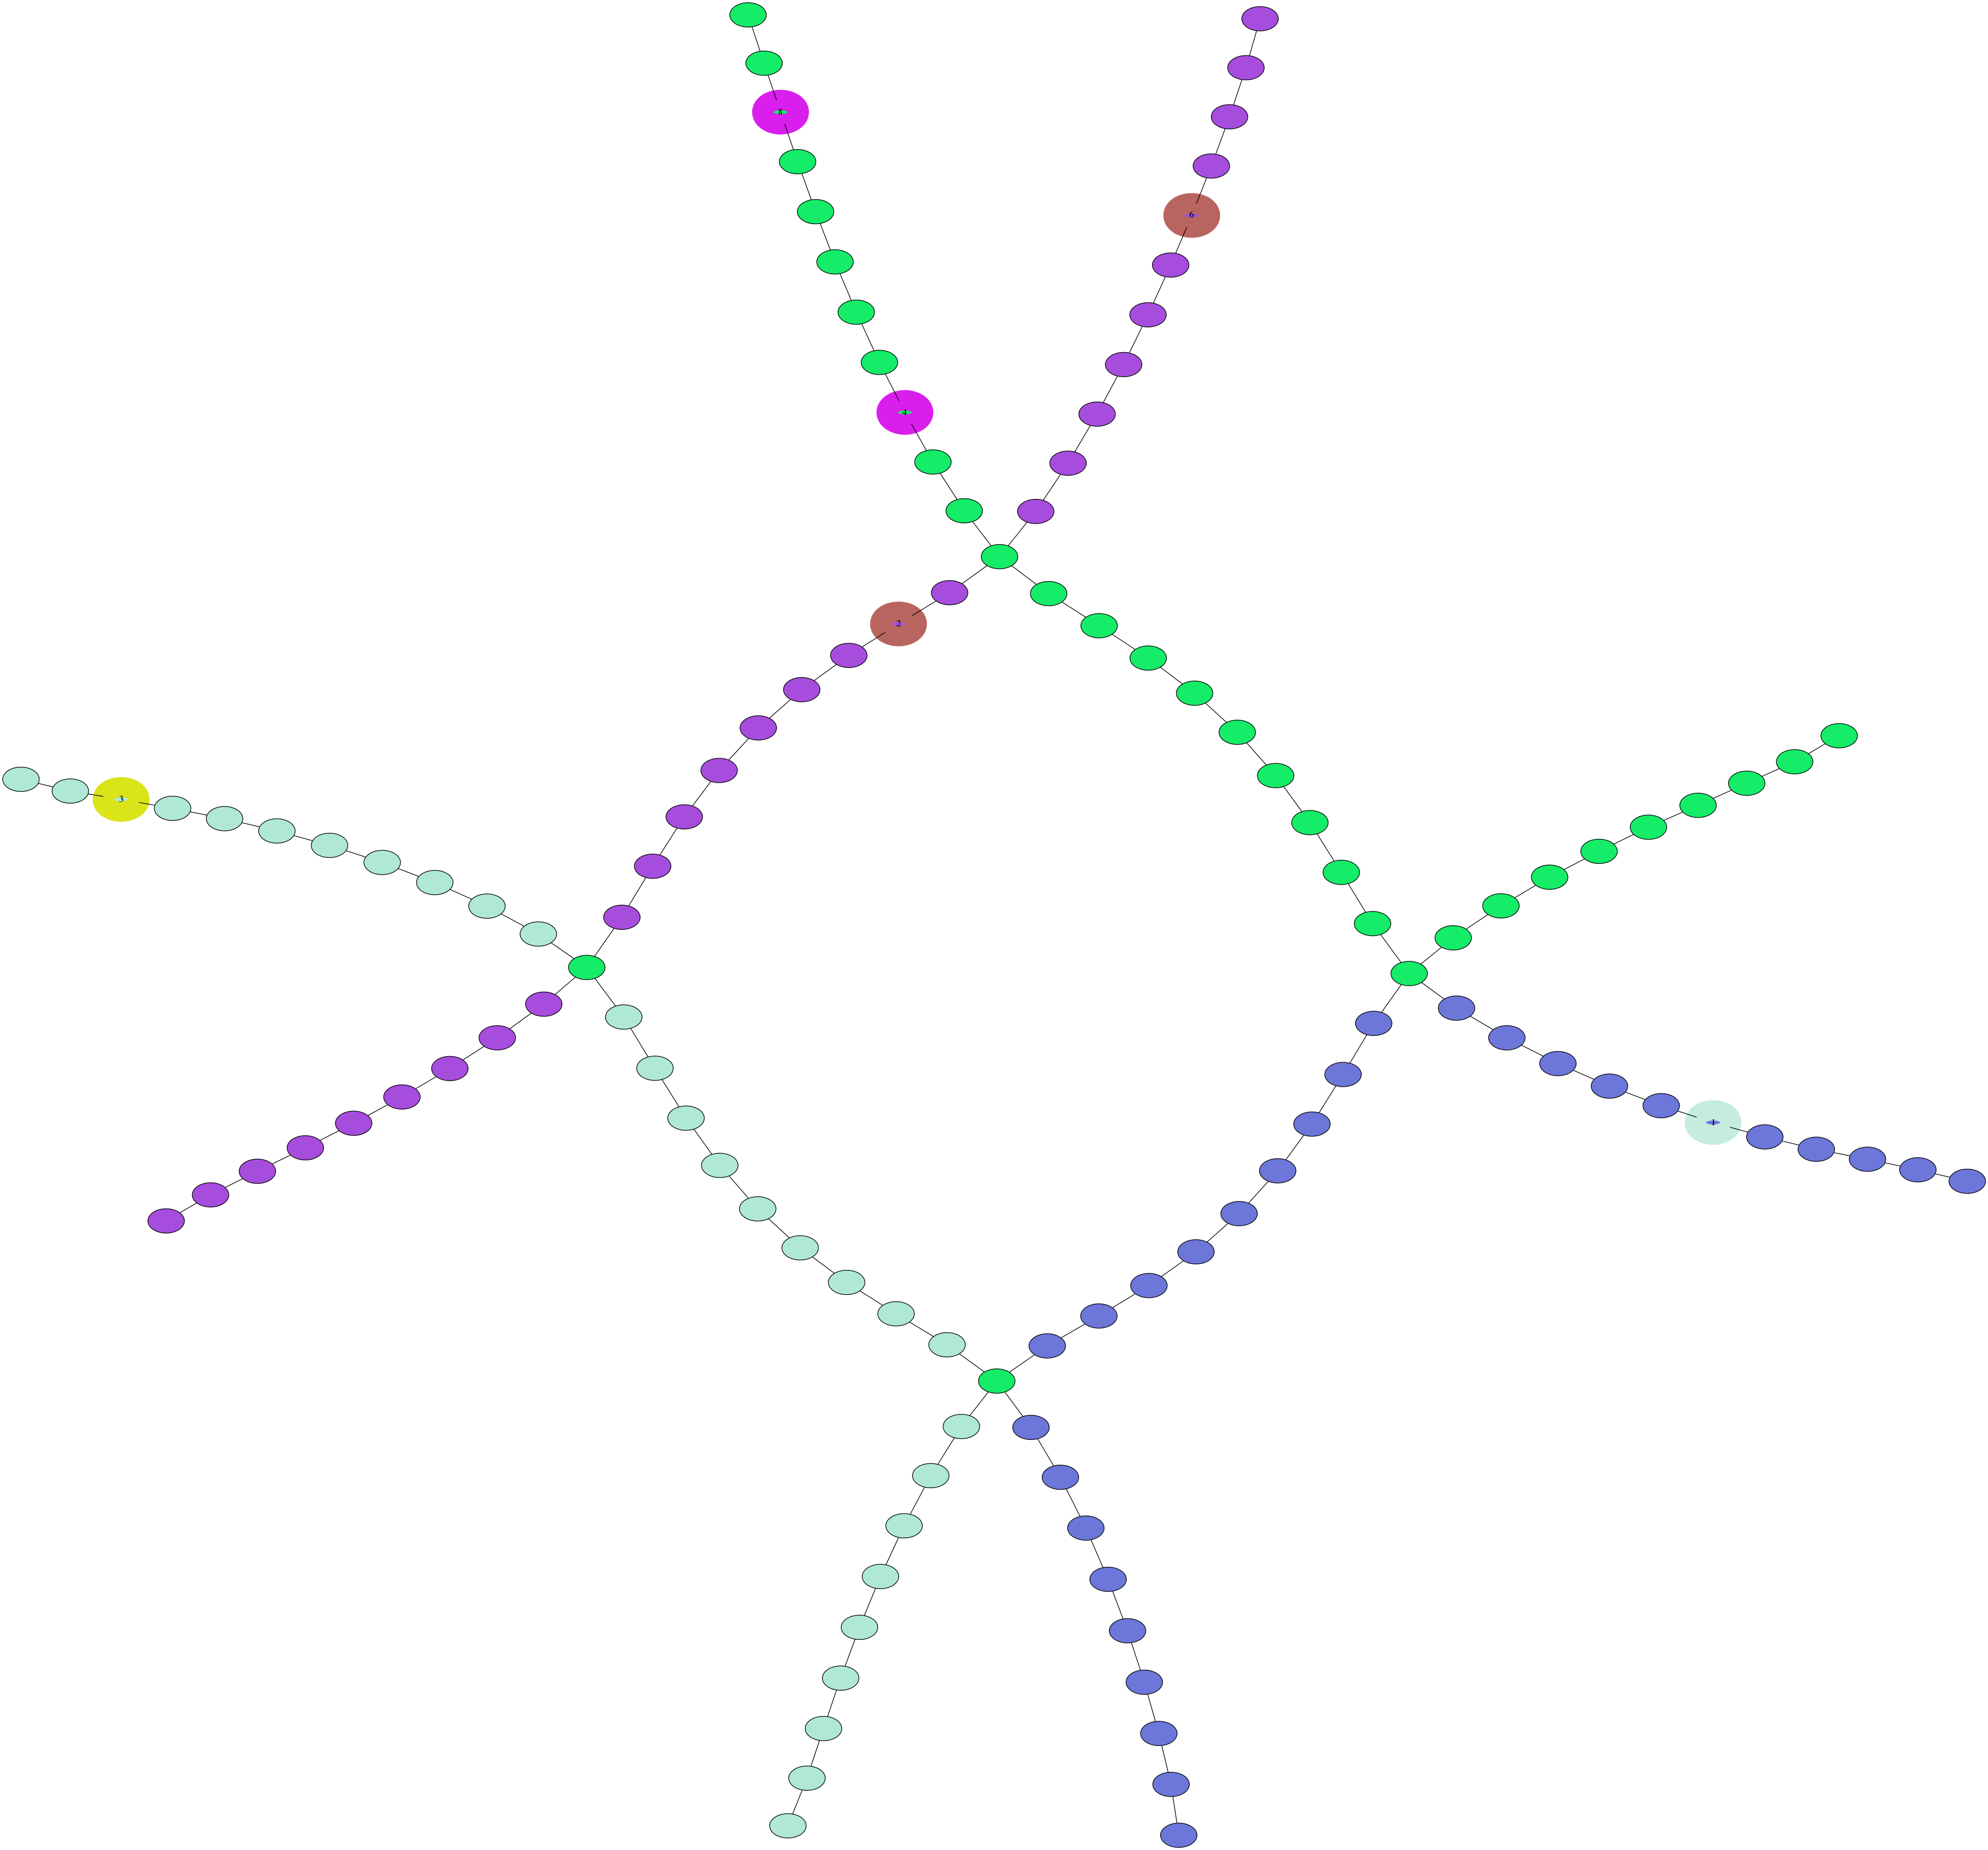
\includegraphics[width=1.0\textwidth]{10.png}
  \caption{10 krok czasowy}
  \label{10-traffic}
\end{figure}
\newpage
\begin{figure}
    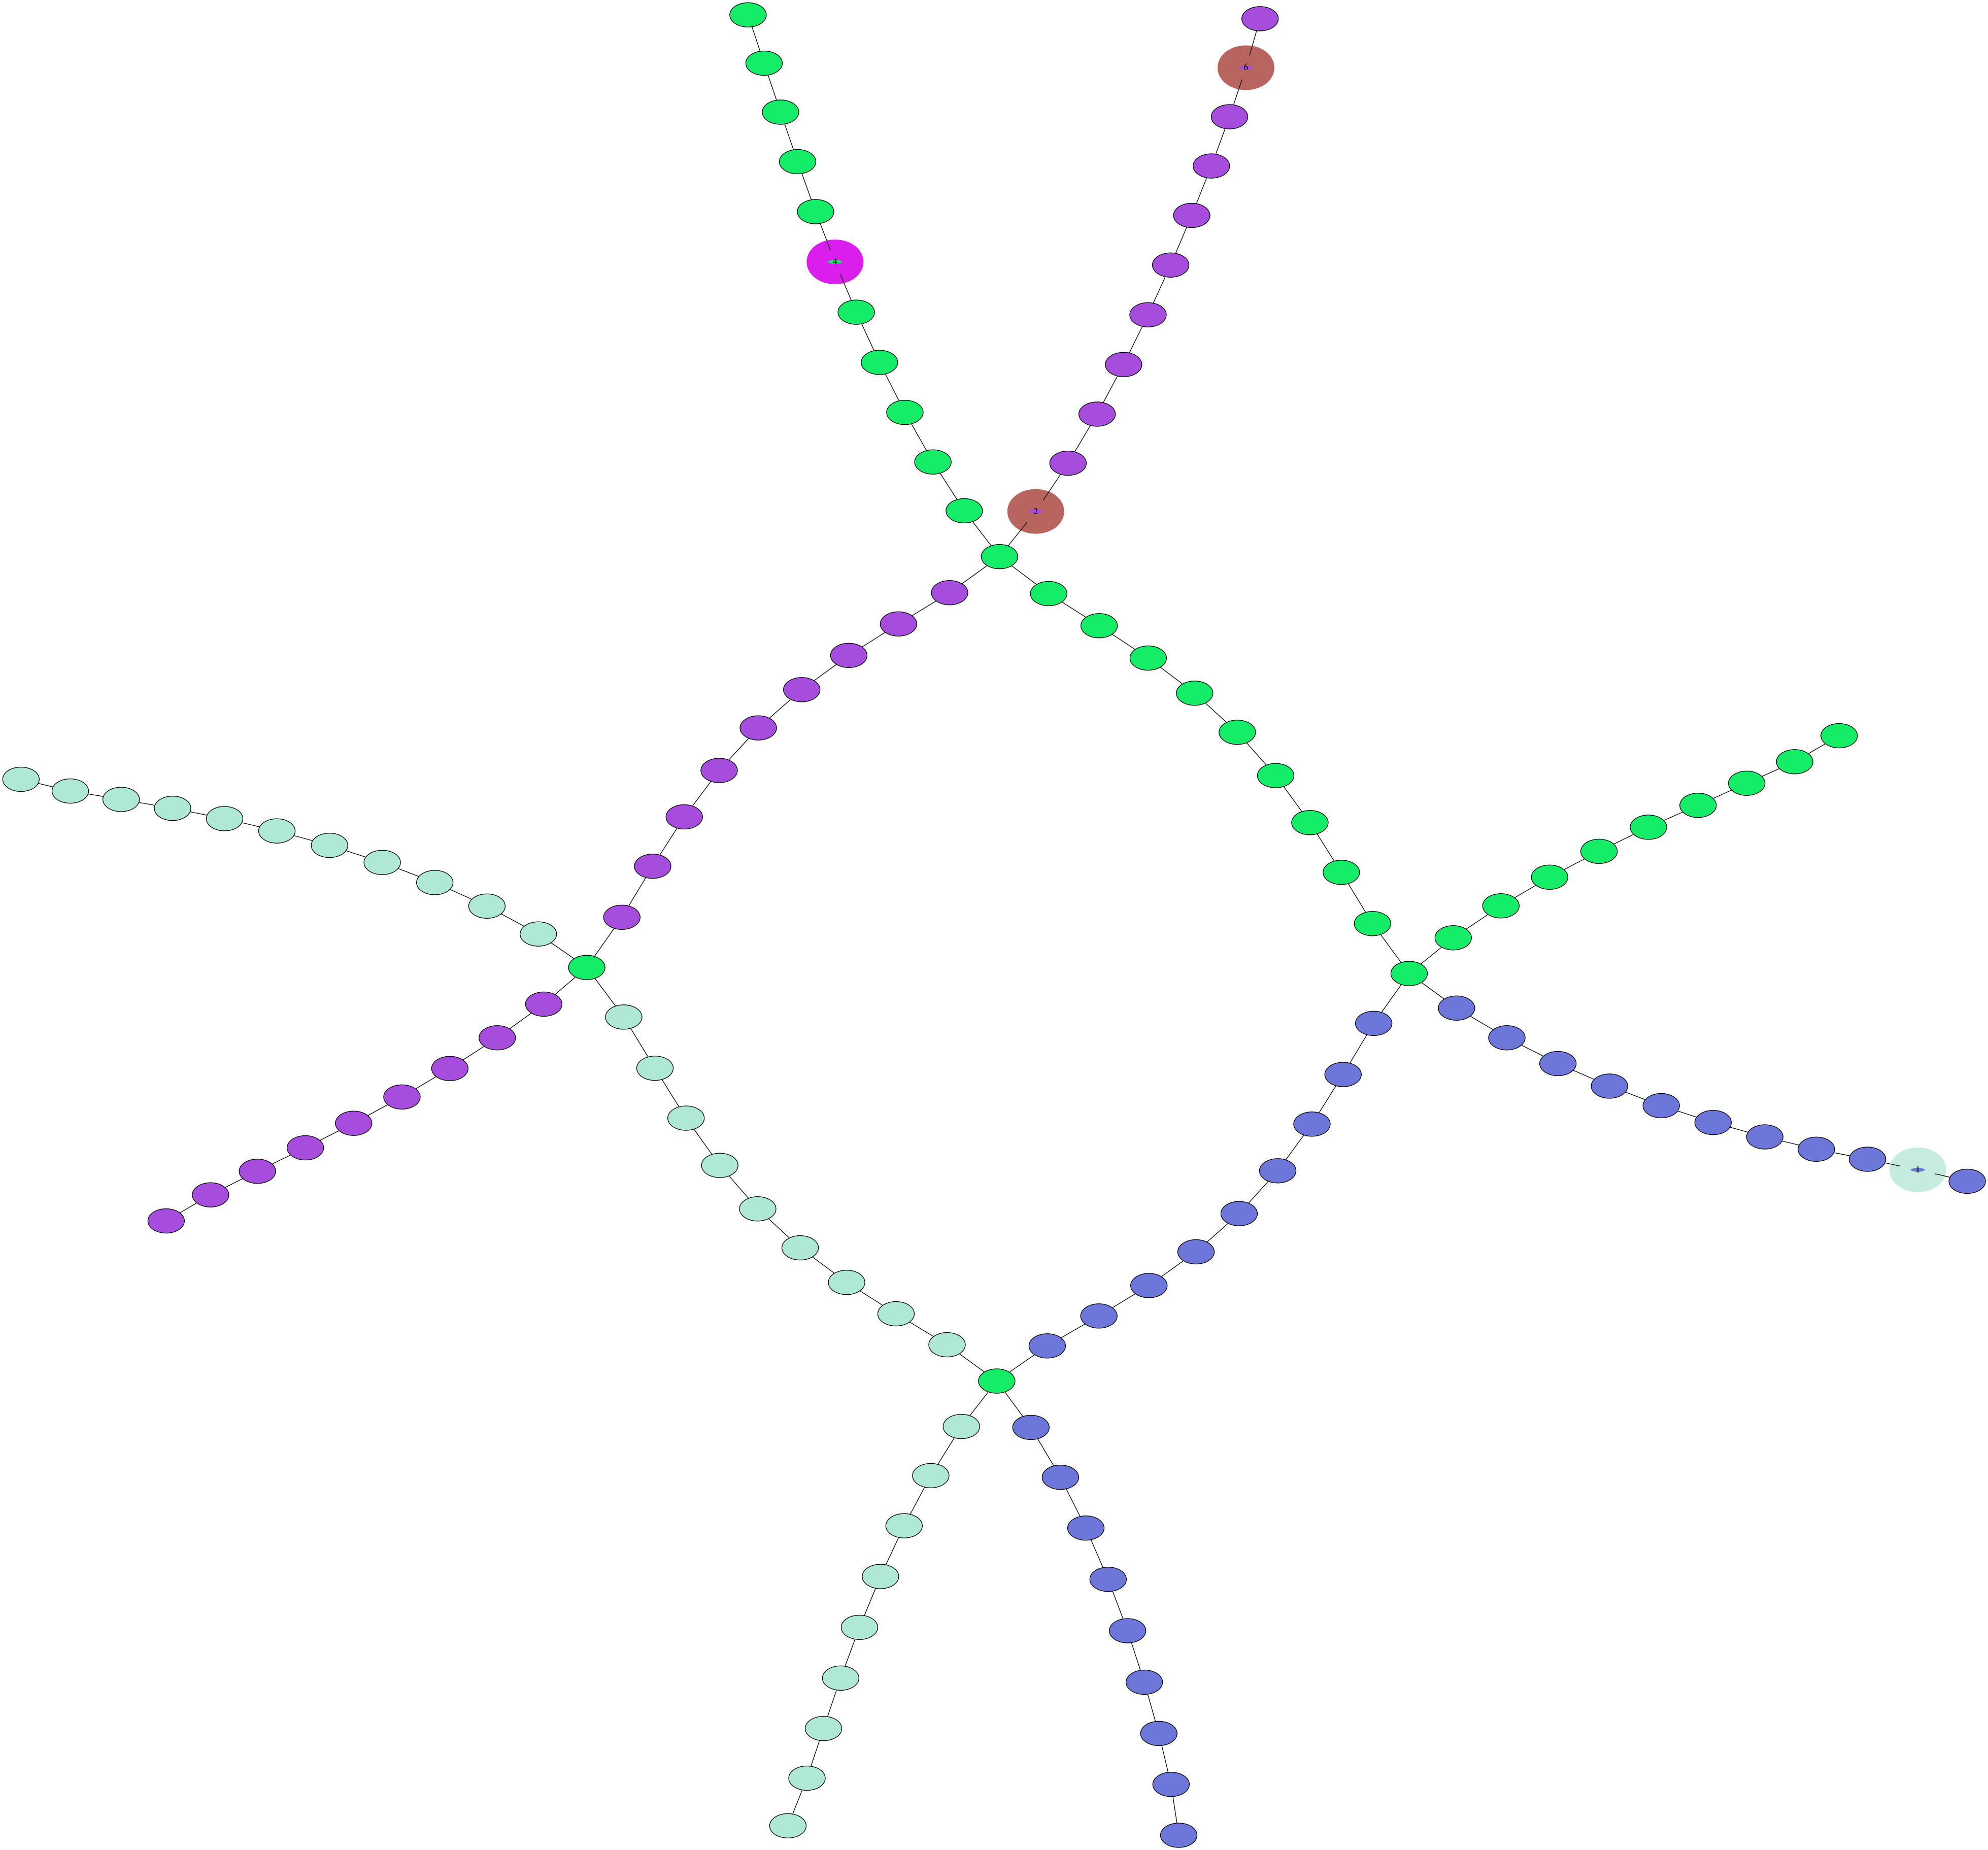
\includegraphics[width=1.0\textwidth]{11.png}
  \caption{11 krok czasowy}
  \label{11-traffic}
\end{figure}
\newpage
\begin{figure}
    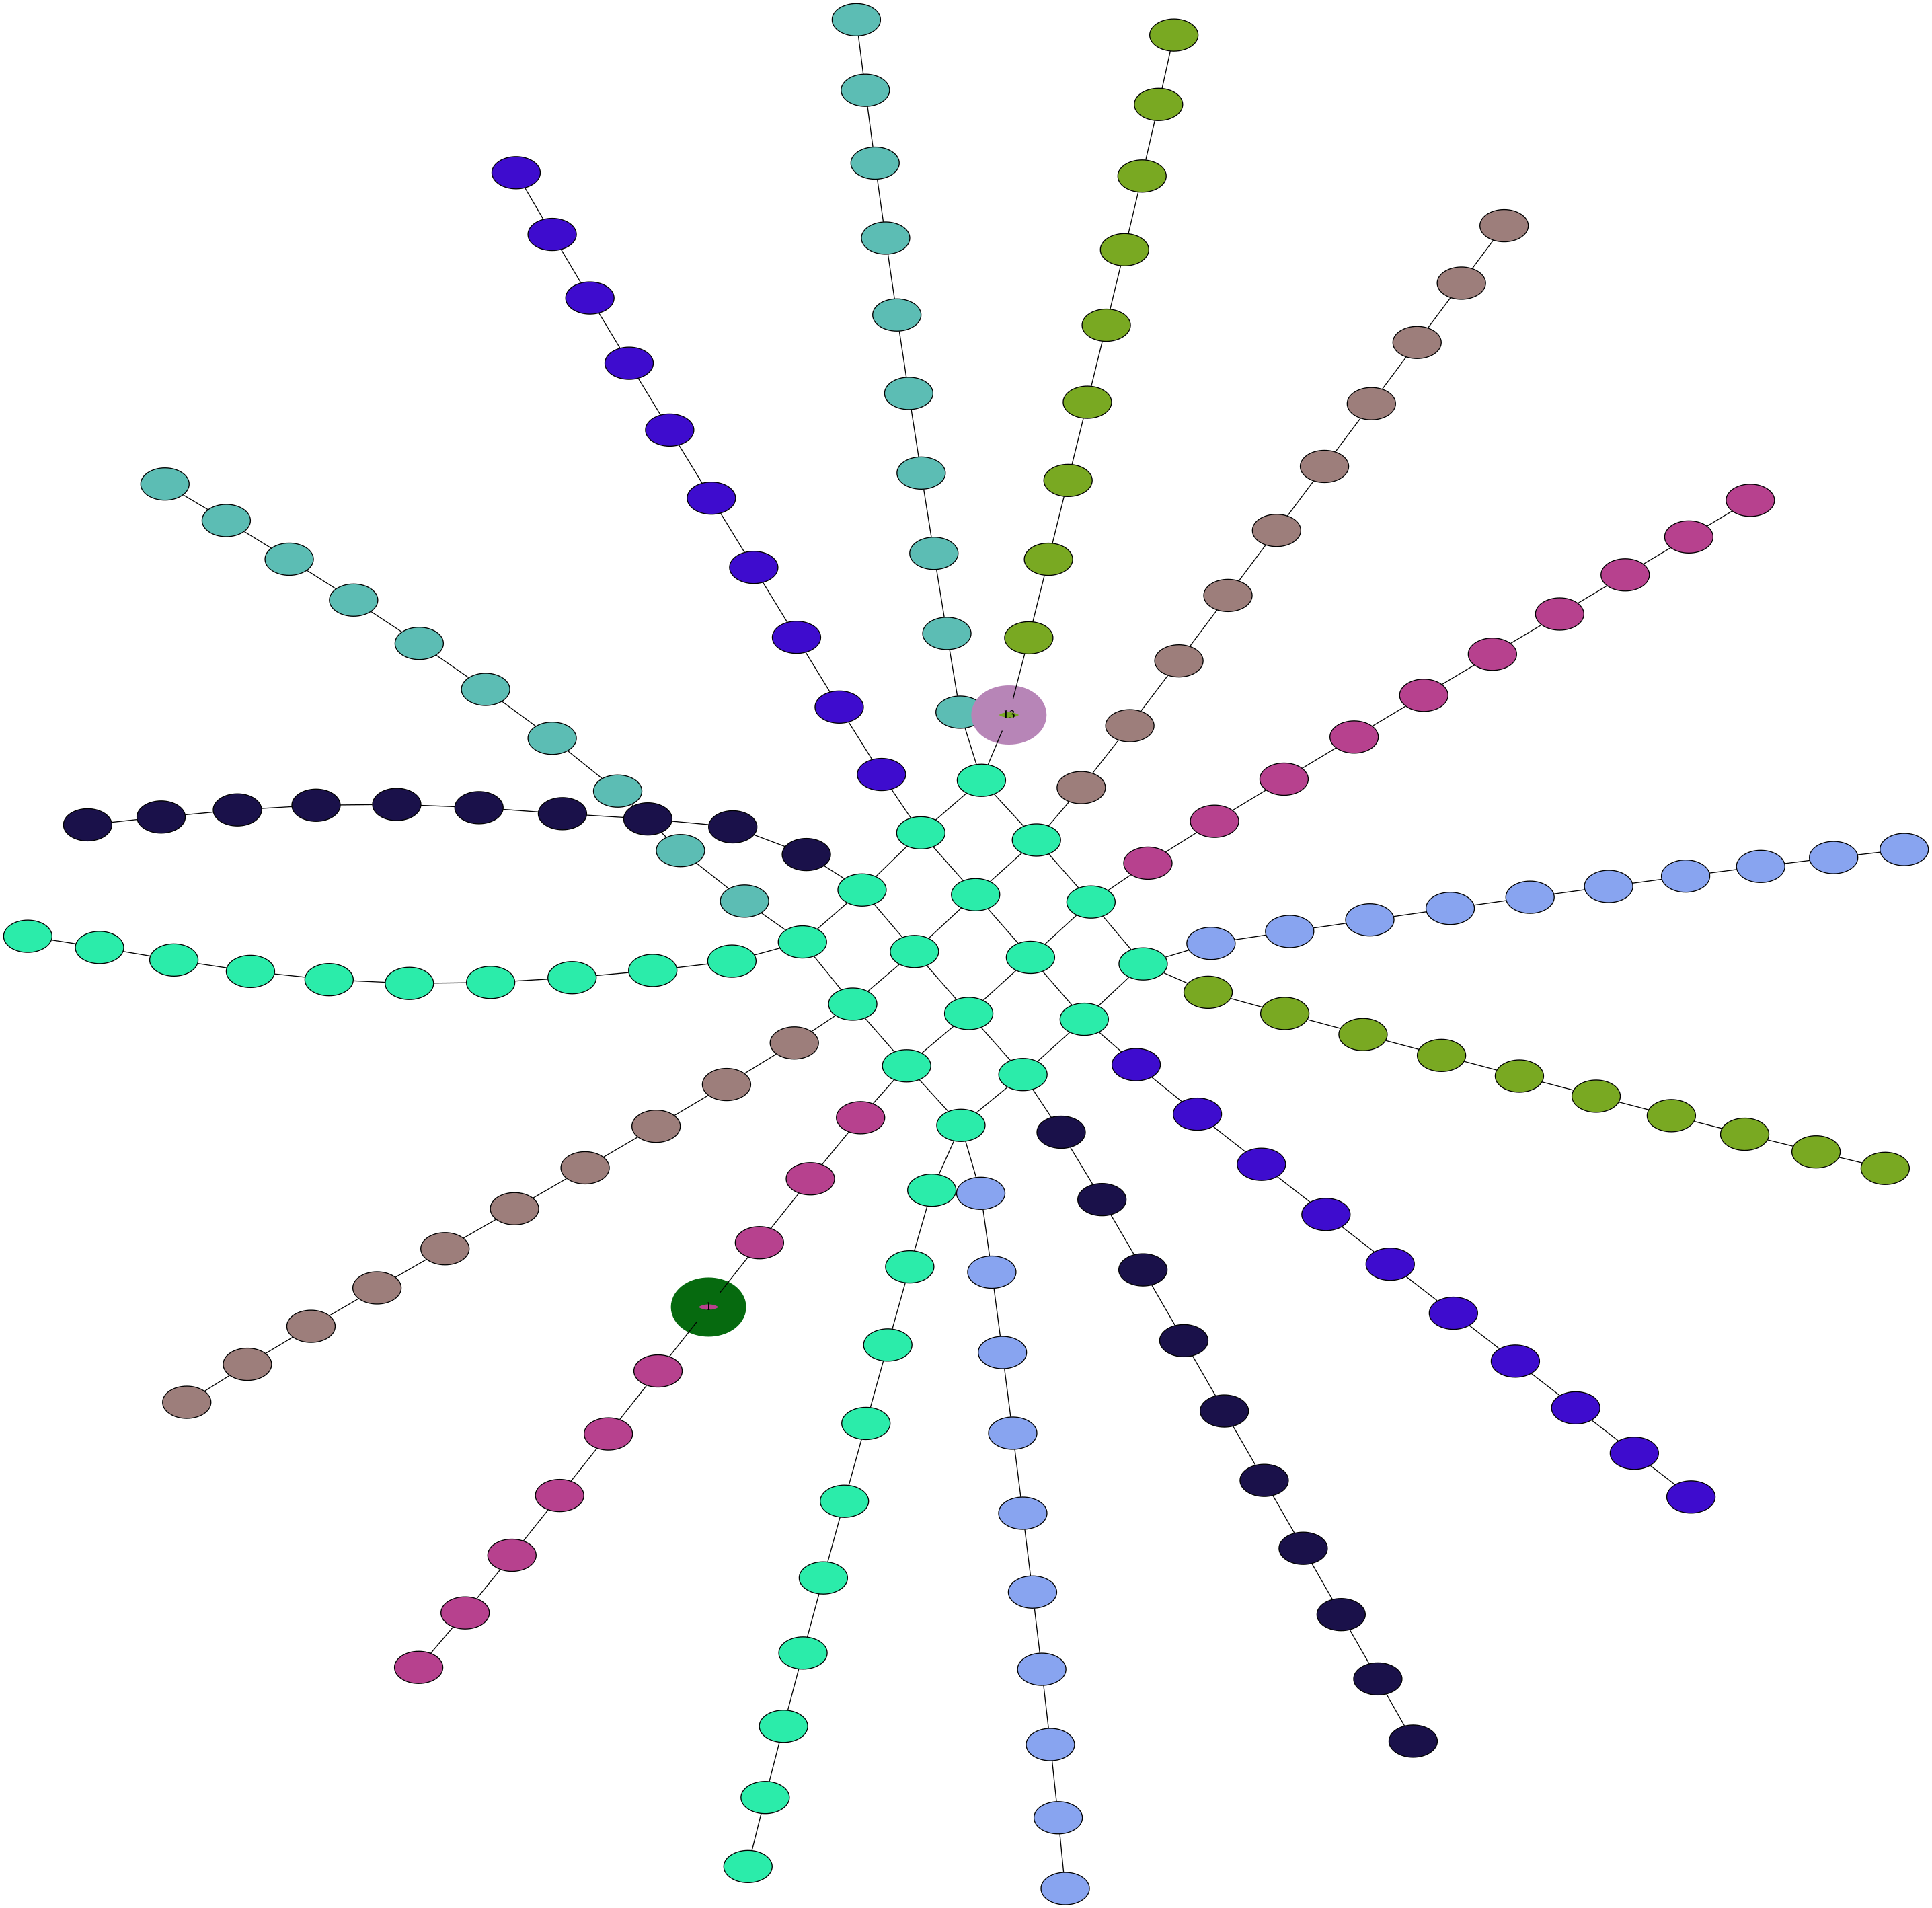
\includegraphics[width=1.0\textwidth]{12.png}
  \caption{12 krok czasowy}
  \label{12-traffic}
\end{figure}
